\chapter{基于运动模型的路面车辆深度视觉里程计}
\label{ch:datavo}
在前两章中,我们分别从损失函数(第\ref{ch:homovo}章)和网络架构(第\ref{ch:padvo}章)两个角度对基于学习的视觉里程计方法进行了改进。而在深度学习算法中,存在关键的三个因素:损失函数、网络架构和训练数据。本章将从路面车辆的运动约束和数据分布的角度对基于学习的视觉里程计模型进行改进。

大部分基于深度学习的视觉里程计算法尝试学习从连续图像对到相机运动的映射模型,其中相机运动一般由三自由度的平移运动和三自由度旋转运动组成。
然而,我们发现,对于路面轮式车辆系统来说,由于运动模式受其自身机械结构的限制和动力机制的约束,其在三维空间的运动并不具备完整的6自由度,大部分运动局限在$Z$轴方向的平移运动和$Y$轴方向的旋转运动(如图\ref{fig:car_simplify}),受限的运动模式进而使网络模型的训练集数据在各个运动维度上分布不均。
\begin{figure}[h]
    \centering
    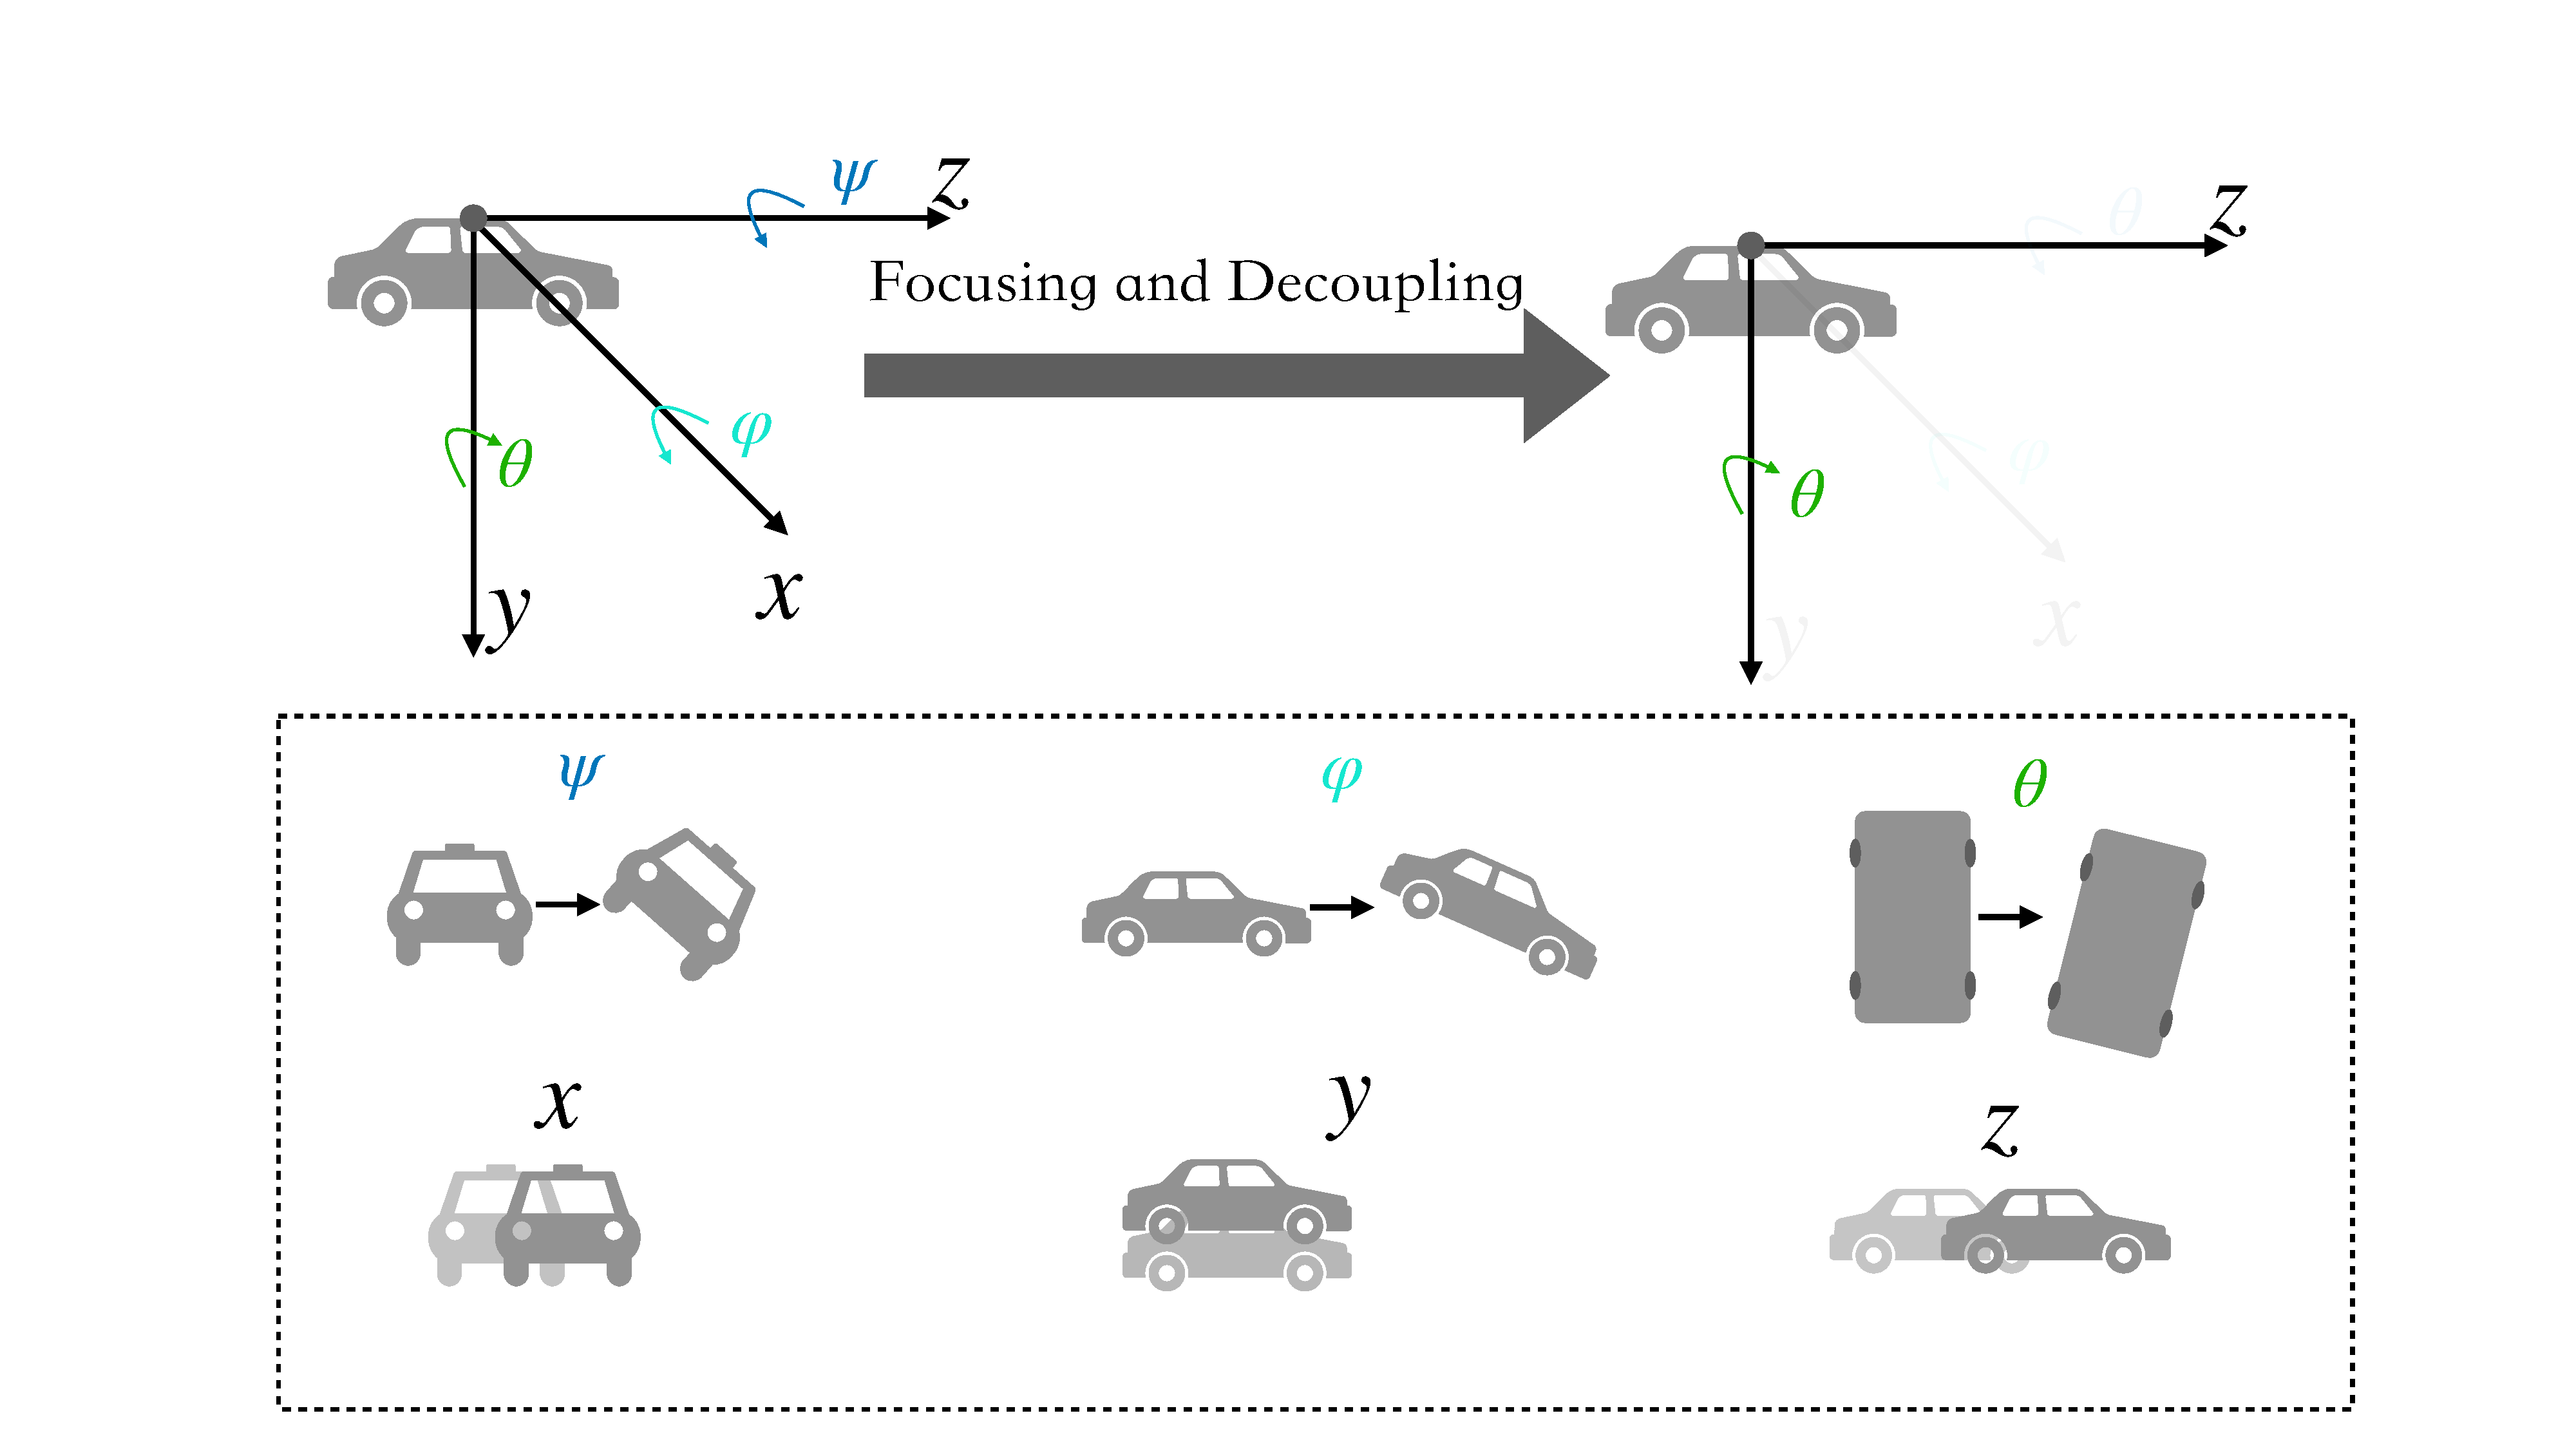
\includegraphics[width=0.95\textwidth]{datavo/car_simplify.pdf}
    \caption{车辆运动简化示意图}
    \label{fig:car_simplify}
\end{figure}
本文认为这是当前基于学习的视觉里程计问题精度较低的原因之一,因为所有基于监督学习的问题都依赖大量的标签数据,如分类问题的Imagenet数据集\cite{deng2009imagenet}和语义分割问题的CityScapes数据集\cite{Cordts2016Cityscapes}。而对于视觉里程计问题,主流的数据集KITTI\cite{geiger2012kitti}在数据量和数据多样性上都存在局限。本章工作基于车辆的运动模型,仅对车辆的主体运动维度进行建模,而忽略运动较小的自由度,并探索运动维度的聚焦和解耦对基于学习的视觉里程计问题的影响。

在基于几何计算的传统视觉里程计问题中,路面车辆的运动模型已经被广泛使用。由于车辆在$Y$轴方向的平移运动幅度极小,固定在车辆上的相机高度
不易发生变化,包括本文第二章在内的很多工作\cite{Song2015MoncularScale,Lee2015MoncularScale,zhou2016reliable,7898840}以此作为绝对尺度参考恢复单目视觉运动估计的绝对尺度。
Scaramuzza等人\cite{scaramuzza2009real}根据车辆Ackermann运动模型,简化车辆运动估计,提出基于单特征点的随机抽样一致进行运动估计,提
高算法实时性。Choi等人\cite{choi2015simplified}在基于路面车辆模型的基础之上,考虑车辆震荡,放松了严格平面运动的约束,使算法更加鲁棒。
此外Scaramuzza等人\cite{4625958}还提出了基于单应性的全景相机视觉里程计。


本章首次将车辆的运动模型引入到基于学习的单目视觉里程计算法中,整体结构如图\ref{fig:datavo_system_structure}。在具体实现上,首先定量评价忽略受限制运动维度所造成的车辆运动轨迹的偏移;然后根据车辆的
旋转运动模型对车辆的旋转运动和平移运动解耦,以减弱在忽略受限制维度运动时的轨迹偏移;
同时本章设计并构建了针对车辆主要运动进行建模的轻量化卷积神经网络模型。基于对上述工作,本章做出如下贡献:
\begin{figure}[h]
    \centering
    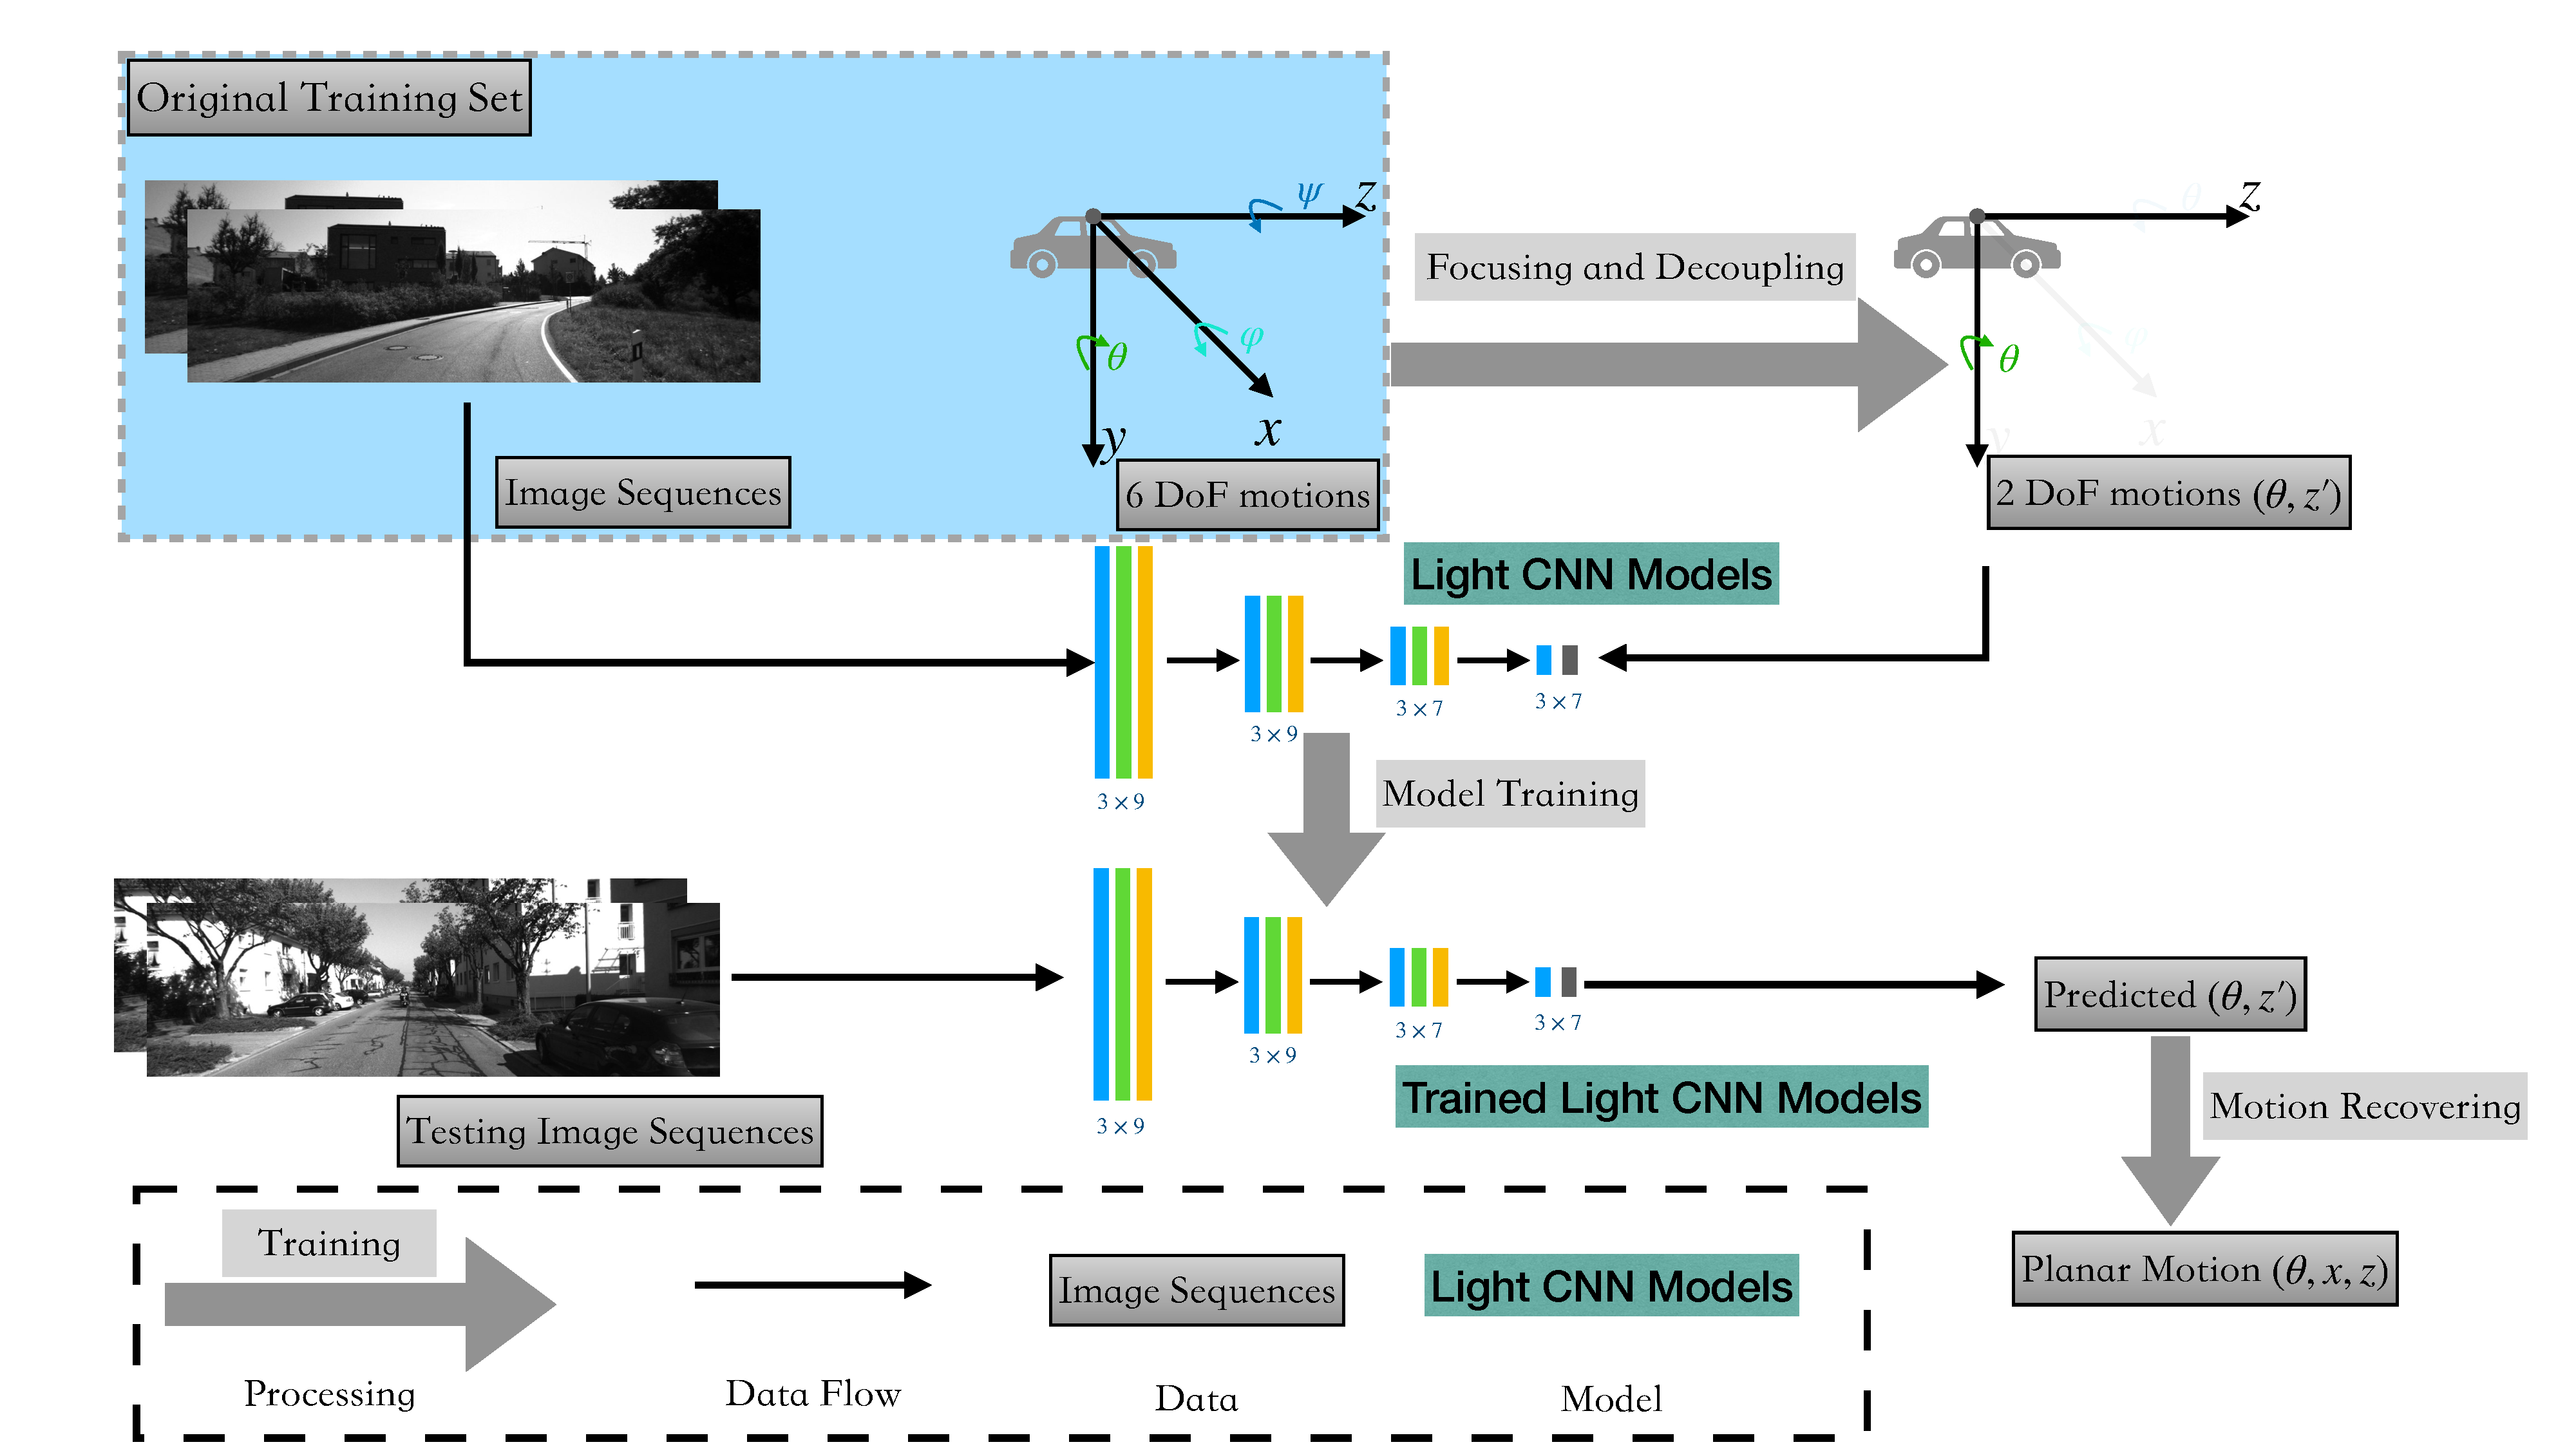
\includegraphics[width=0.95\textwidth]{datavo/system_structure.pdf}
    \caption{路面车辆视觉里程计映射学习系统架构图}
    \label{fig:datavo_system_structure}
\end{figure}
\begin{enumerate}
    \item 本章通过实验定量地分析了运动聚焦所造成的轨迹偏移,并证明了运动聚焦的可行性;
    \item 本章根据车辆的运动模型,分析了车辆沿$X$轴的平移运动与绕$Z$轴旋转运动之间的映射关系,并通过运动解耦减低了运动聚焦时的运动偏移;
    \item 本章实验证明了运动聚焦和运动解耦可以提高基于学习的单目视觉里程计的性能,包括减少训练时间、提升训练精度;
    \item 本章构建了一个十分轻量化的运动估计网络,该网络在训练时仅需占用2G的图形处理单元(GPU)显存并可以快速收敛,并可以在取得与其它算法可比精准度的前提下以200帧每秒的速度实时运行在CPU上,算法已开源\footnote{https://github.com/TimingSpace/DMVOGV}.
\end{enumerate}

本章结构如下:
首先在第\ref{sec:motion}节介绍算法的数学原理和实现方式;然后在第\ref{sec:datavo_experiments}节,我们在KITTI数据集\cite{geiger2012kitti}定性和定量的评价我们算法;
最后在\ref{sec:datavo_conclusion}节总结本章工作。

\section{路面车辆视觉里程计方法}
运动聚焦,即忽略车辆运动维度较小的维度,聚焦于车辆的主体运动。根据车辆模型的约束,以简化运动估计为目的,本章提出了运动聚焦算法,并通过运动解耦算法以降低运动聚焦带来的位姿偏移。
本节,我们首先在第\ref{sec:motion}节介绍运动聚焦和运动解耦方法;然后在第\ref{sec:model}节介绍模型架构以及训练和测试方法。
%\subsection{Data Processing}

\subsection{运动聚焦与解耦}
\label{sec:motion}

\begin{figure}[ht]
    \centering
    \begin{subfigure}[b]{0.48\textwidth}
        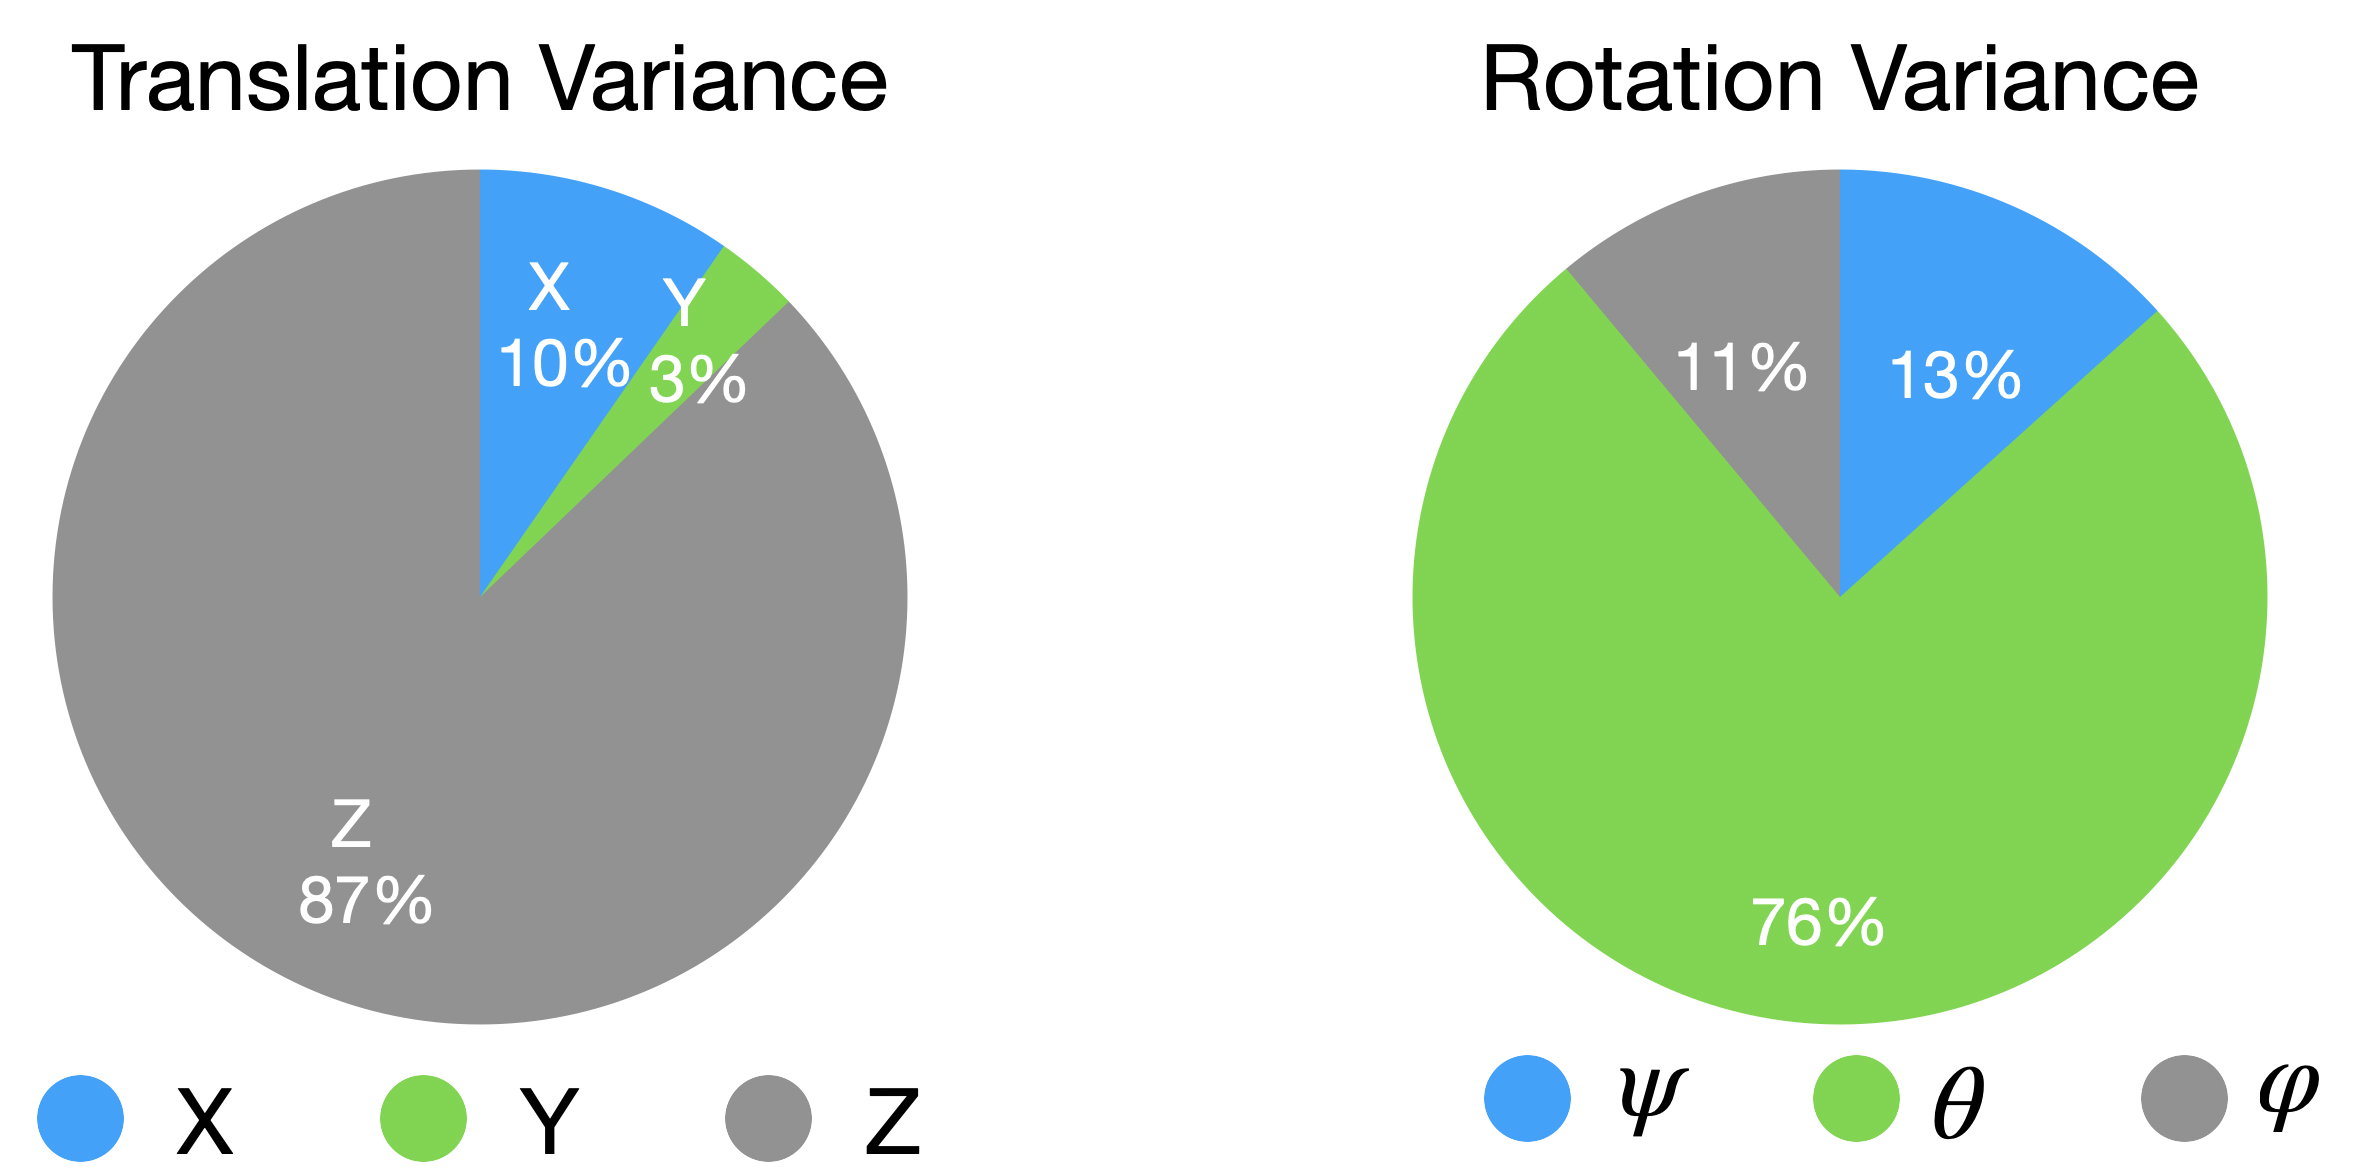
\includegraphics[width=\textwidth]{datavo/motion_dis.png}
        \caption{运动分布}
        \label{fig:motion_dis} 
    \end{subfigure}
    \begin{subfigure}[b]{0.48\textwidth}
        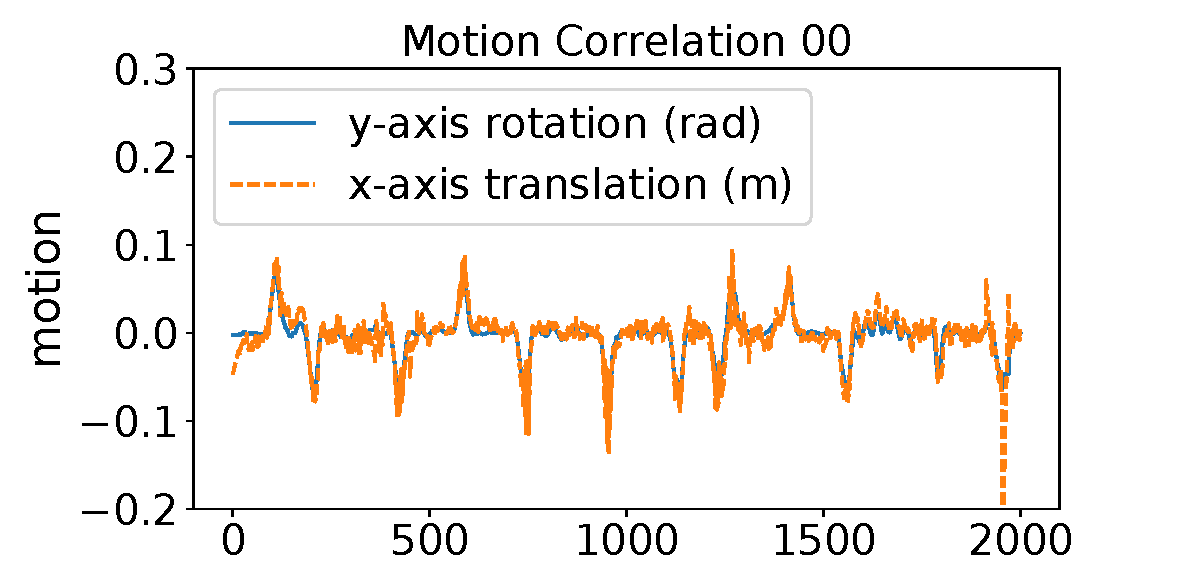
\includegraphics[width=\textwidth]{datavo/rotation_corr.pdf}
        \caption{运动耦合}
        \label{fig:rotation_corr}
    \end{subfigure}
    \caption{路面车辆运动模态分析}

\end{figure}
\subsubsection{运动聚焦}
根据车辆的机械结构和动力模型的限制,车辆的主要运动为沿$Z$轴的平移运动(前进)和绕$Y$轴的旋转运动(转向)。KITTI视觉里程计数据集中车辆在各个维度上的运动方差给这一论点提供了数据支撑,如图\ref{fig:motion_dis}所示(此图中仅可视化了KITTI数据集00序列的运动,为了说明其代表性,附录\ref{ch:app_motion_dis}中可视化了更多的数据)。运动表征选择使用标准的相机坐标系,其为以相机光心为原点的右手坐标系,向前为$Z$轴方向,向右和向下分别$X$轴方向和$Y$轴方向。车辆绕$X$轴、$Y$轴和$Z$轴的旋转运动的欧拉角分别表示为 $\psi$, $\varphi$和 $\theta$。从图\ref{fig:motion_dis}中可看出,车辆的平移运动确实主要集中在$Z$轴方向,而车辆的旋转运动主要集中在$Y$轴上,所以本章选择仅建模输入图像到车辆$Z$轴平移运动和$Y$轴旋转运动的映射,这个过程称之为为运动聚焦。
\begin{figure}[ht]
    \centering
    \begin{subfigure}[b]{0.48\textwidth}
        \centering
        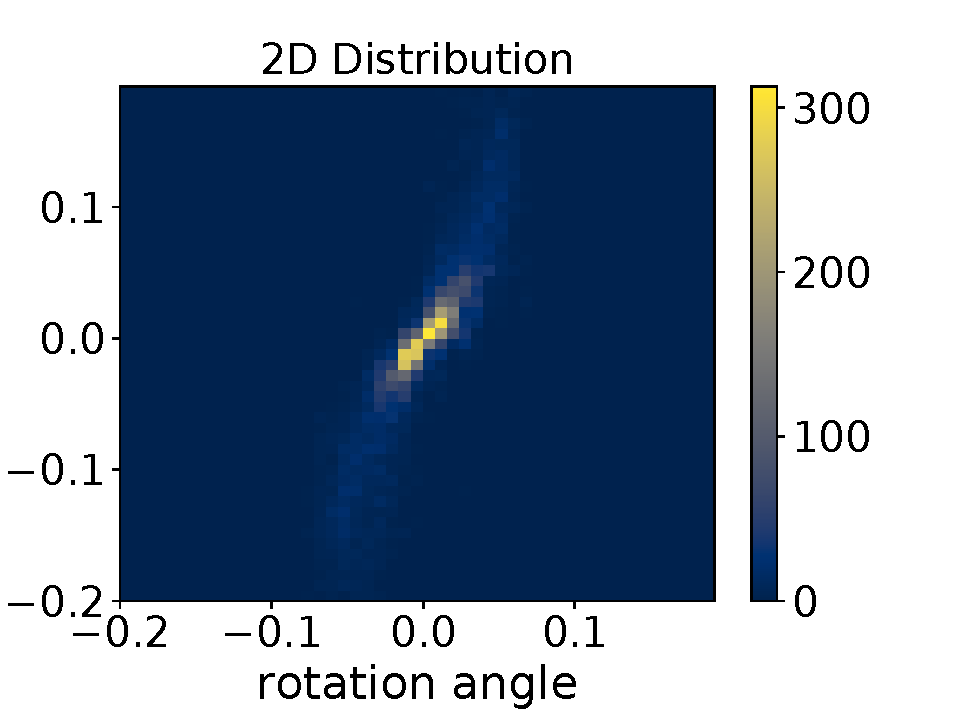
\includegraphics[width=\textwidth]{datavo/r_t_2d_hist.pdf}
        \caption{二维联合分布}
        \label{fig:rt_2d} 
    \end{subfigure}
    \begin{subfigure}[b]{0.48\textwidth}
        \centering
        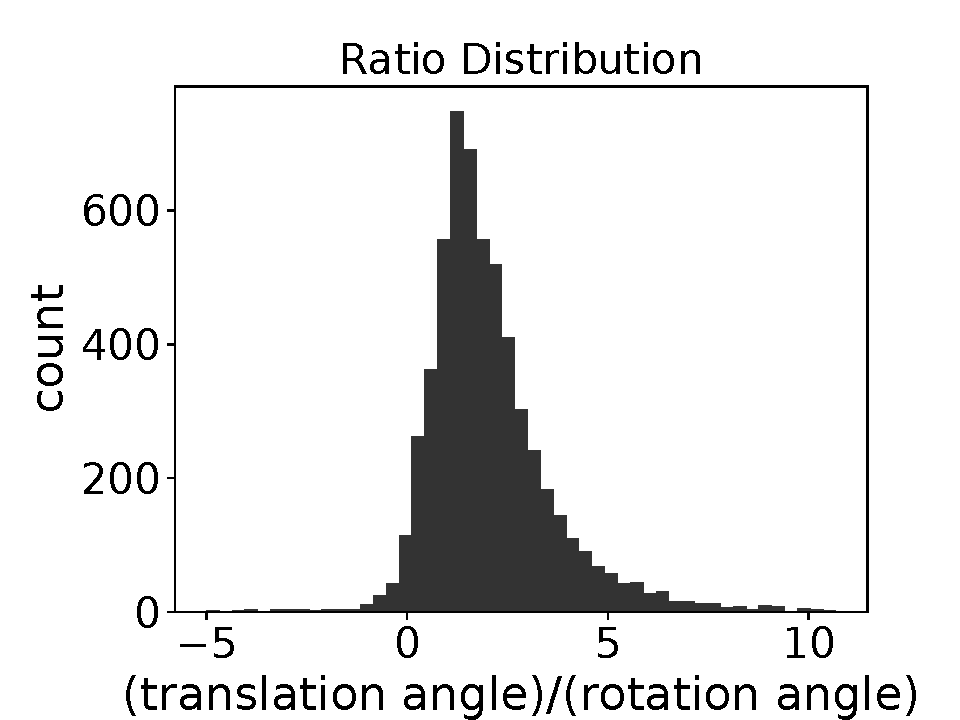
\includegraphics[width=\textwidth]{datavo/r_t_1d_hist.pdf}
        \caption{比例分布}
        \label{fig:rt_1d}
    \end{subfigure}
    \caption{$X$轴平移运动与$Y$轴旋转运动的相关性}
    \label{fig:rotation_corr_analysis}
\end{figure}

\subsubsection{运动解耦}
然而,我们发现车辆依然存在着一定幅度(约10\%)的$X$轴平移运动(如图\ref{fig:motion_dis})。但由于动力约束,路面车辆系统从原理上是无法沿$X$轴有大幅度的运动的,那么这10\%的轴平移运动来自哪里呢?
通过仔细分析无人车的旋转模式可知$X$轴的平移运动产生的原因为车辆的运动表征方式:

\begin{equation}
    \begin{pmatrix} \mathbf{R} & \mathbf{t}\\ 0 & 1  \end{pmatrix} = \begin{pmatrix} \mathbf{I}& \mathbf{t}\\ 0 & 1  \end{pmatrix}\begin{pmatrix} \mathbf{R}& \mathbf{0}\\ 0 & 1  \end{pmatrix}
    \label{eq:ftlr}
\end{equation}
其中
$\mathbf{I}$ 为3x3的单位矩阵。 
在这种表征方式中,机器人首先进行相对于初始基坐标系平移运动$\mathbf{t}$,然后在运动之后的基坐标系上进行旋转运动$\mathbf{R}$(基坐标系指机器人自身坐标系)\cite{sun1995robot},那么如果机器人同时进行了旋转和平移运动,继而车辆的参考坐标系会因为旋转运动发生变化,本来仅沿
$Z$轴的平移运动也会由于旋转的存在映射成$Z$轴平移分量与$X$轴平移分量,如图\ref{fig:rotation_model}所示。参考坐标系变化带来的平移偏角$\alpha$定义为:
\begin{equation}
    \alpha = \arctan\left(\frac{x}{z}\right)
\end{equation}
其中$x$和$z$分别表示$X$轴和$Z$轴的平移运动。
从图\ref{fig:rotation_corr}中可以看出,$X$轴的平移运动与$Y$轴的旋转运动相关性
很强,这一点恰好证明$X$轴运动源自于旋转后运动映射。由于图\ref{fig:rotation_corr}只能评价局部的运动相关性,为了得到更具代表性的结果,我们通过直方图可视化旋转角度$\theta$和平移偏角$\alpha$的全局关系。 图\ref{fig:rt_1d}的一维直方图可视化了$\alpha/\theta$的分布曲线;图\ref{fig:rt_2d}中的二维直方图可视化了$\alpha$和$\theta$的联合概率分布。从两个直方图中都可以看出,车辆旋转角$\theta$和平移偏角$\alpha$有着很强的相关性。

那么如何通过改变运动表征方式来解除$X$轴平移运动与$Y$轴旋转运动之间的耦合呢?一种朴素的方法为调换旋转
运动和平移运动的顺序,车辆先进行旋转运动,然后在旋转之后的坐标系下进行平移运动,这样车辆的平移运动就不会被映射到$X$轴上,这种运动表征方式可以公式化为:
\begin{equation}
    \begin{pmatrix} \mathbf{R} & \mathbf{t}\\ 0 & 1  \end{pmatrix} = \begin{pmatrix} \mathbf{R'}& \mathbf{0}\\ 0 & 1  \end{pmatrix}\begin{pmatrix} \mathbf{I}& \mathbf{t'}\\ 0 & 1  \end{pmatrix}
    \label{eq:frlt}
\end{equation}
可以推出公式中
$\mathbf{R'} = \mathbf{R}$, $\mathbf{t'} = \mathbf{R}^{-1}\mathbf{t}$,相当于把由于旋转重映射的平移运动再反映射回来。
\begin{figure}[ht]
    \centering
    \begin{subfigure}[b]{0.48\textwidth}
        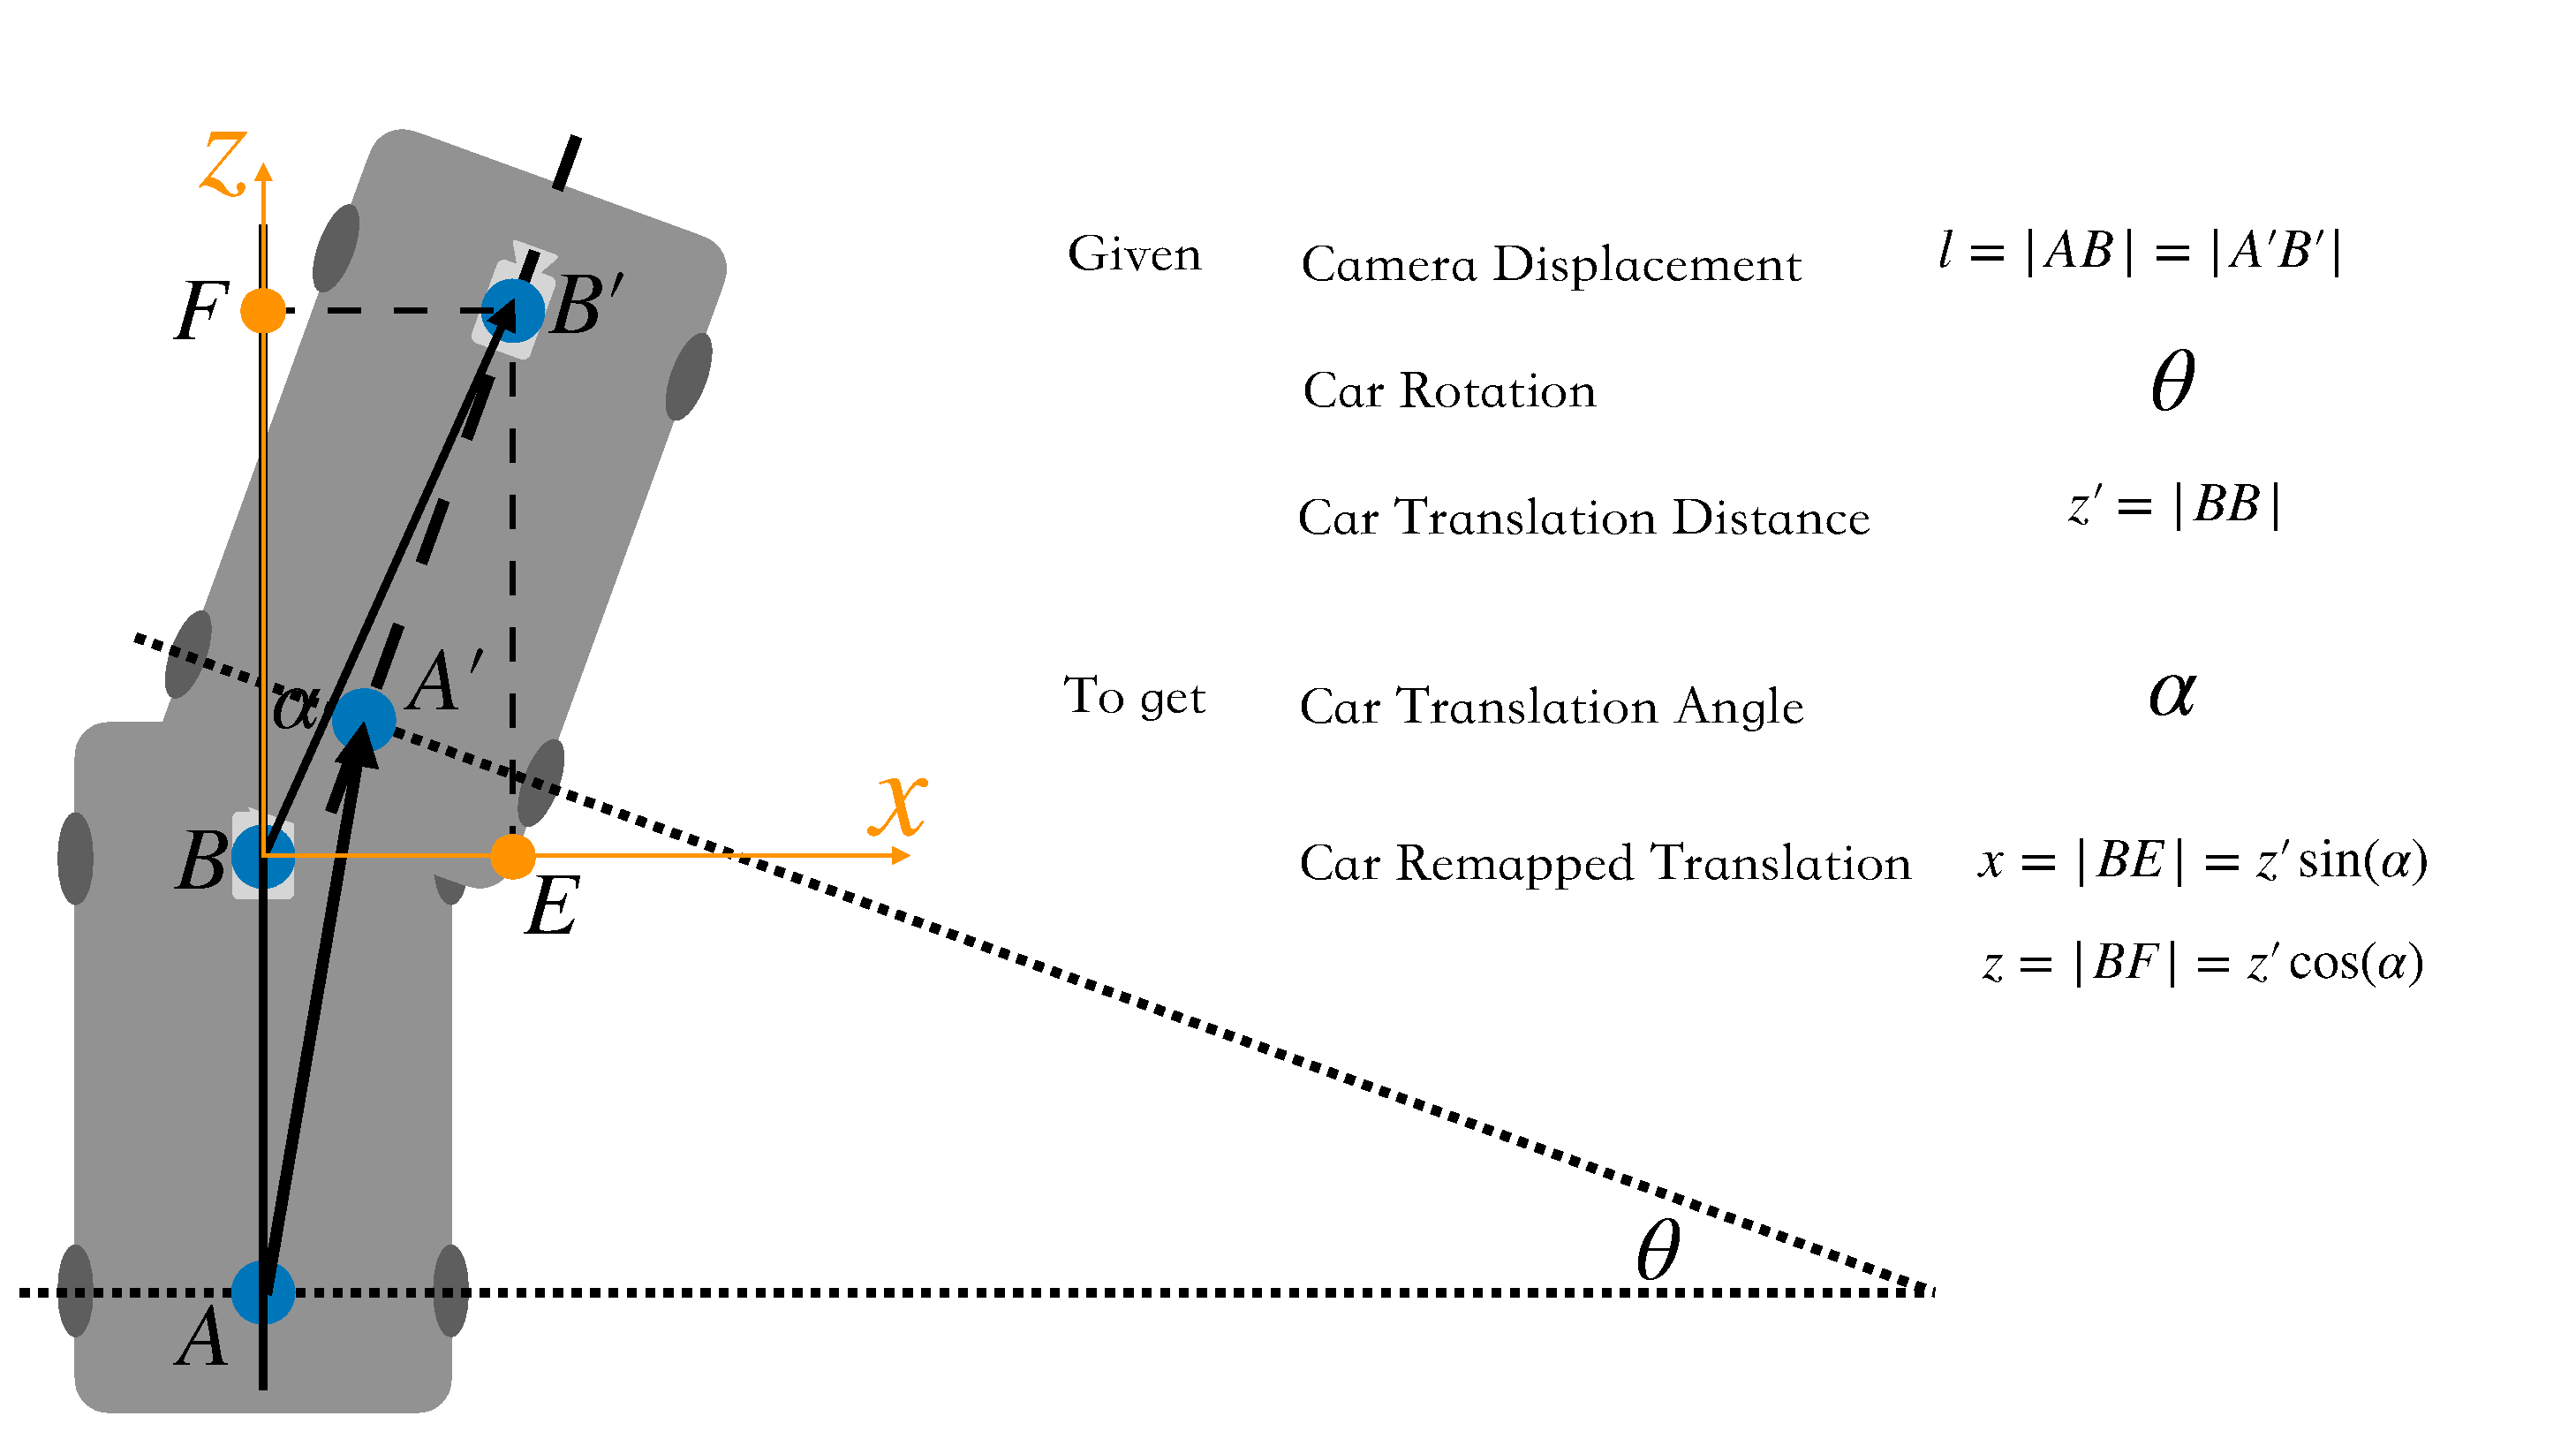
\includegraphics[width=\textwidth]{datavo/vehicle_rotation_1-crop.pdf}
        \caption{车辆旋转示意图}
        \label{fig:vehicel_rotation_model} 
    \end{subfigure}
    \begin{subfigure}[b]{0.48\textwidth}
        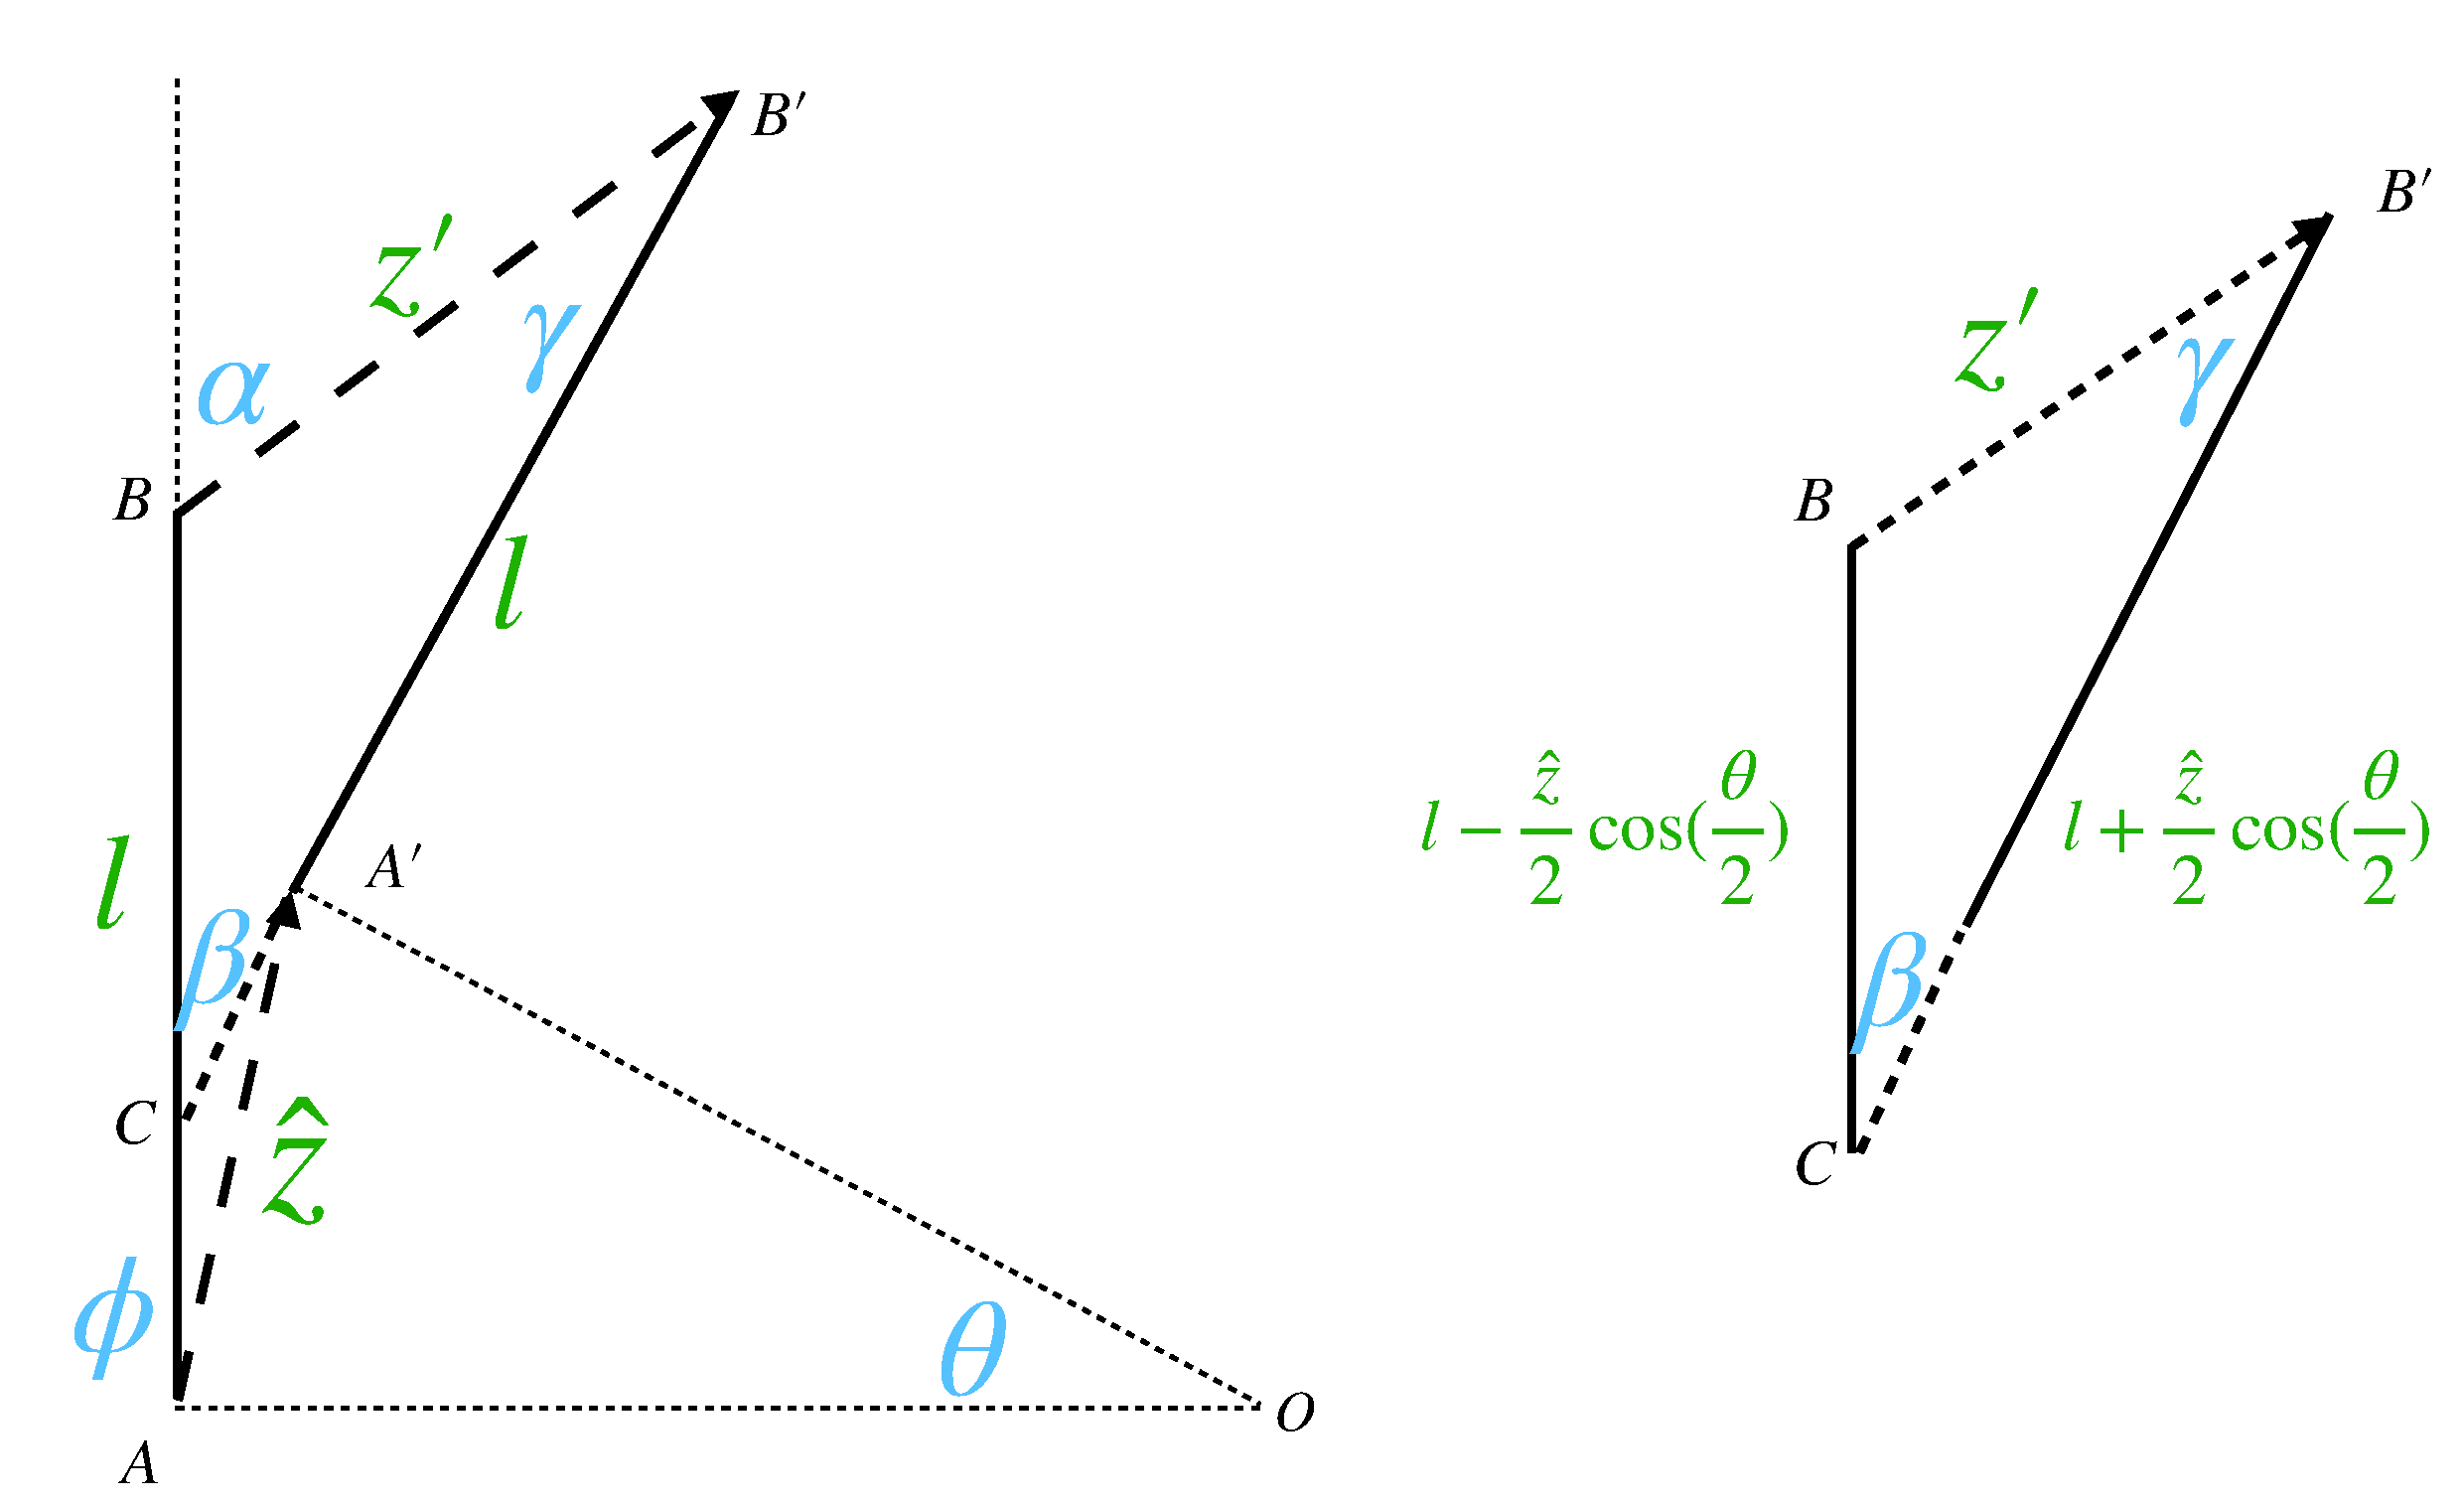
\includegraphics[width=\textwidth]{datavo/vehicle_rotation_2-crop.pdf}
        \caption{简化版示意图}
        \label{fig:vehicel_rotation_model_s} 
    \end{subfigure}
    \caption{车辆旋转模型示意图}
    \label{fig:rotation_model}
\end{figure}
然而,如图\ref{fig:vehicel_rotation_model}所示,由旋转运动引发的车辆平移偏角$\alpha$其实并不等于车辆的旋转角$\theta$。重映射依赖于平移偏角$\alpha$与旋转角$\theta$ 之间的关系,我们定义其间关系为$\alpha = f(\theta)$。在已知这个关系的基础之上,可以
使用车辆的前进距离和车辆的旋转角这两个运动参数来表征车辆的平面运动,平面运动中的平移运动为
\begin{equation}
    (x,z) = z(sin(f(\theta)),cos(f(\theta)))
    \label{eq:car_angle}
\end{equation}

图\ref{fig:vehicel_rotation_model}中,A点表示车辆后轴的中心,B点表示相机的安装位置,设定A点和B点之间的距离为$l$,称之为相机偏距。
视觉里程计之间估计的运动为B点和B'之间的距离,记为$z'$。我们将图\ref{fig:vehicel_rotation_model}简化为图\ref{fig:vehicel_rotation_model_s}。

根据车辆Ackermann运动模型\cite{siegwart2011introduction},$OA \bot AB$ 且 $OA' \bot A'B'$,于是可以得到 $\phi = 0.5 \beta = 0.5 \theta$。
在三角形$CBB'$中,根据正弦定理:
\begin{equation}
    \frac{\sin(\gamma)}{\sin(\beta)}  = \frac{l-\frac{\hat{z}}{2} / \cos(\frac{\theta}{2})}{z'} 
 \end{equation}
考虑到$\theta$的绝对值很小且接近0, 可做如下近似 $\cos(\frac{\theta}{2}) \approx 1$ 且 $ \frac{\gamma}{\beta} \approx  \frac{\sin(\gamma)}{\sin(\beta)} $,于是
\begin{equation}
    \frac{\gamma}{\beta}  \approx \frac{l-\frac{\hat{z}}{2}}{z'} 
\end{equation}
记$d = |AC| \approx 0.5|AA'| =0.5\hat{z}$, 在三角形$CBB'$中根据余弦定理:
\begin{equation}
    z'^2 = (l+d)^2 + (l-d)^2- 2(l+d)(l-d)\cos(\beta) = 2l^2+2d^2 - 2(l^2-d^2)\cos(\beta)\approx 4d^2
\end{equation}
所以 $z'\approx \hat{z}$.
最后可得到了平移偏角$\alpha$和旋转角$\theta$之间的关系
\begin{equation}
    \alpha = \beta + \gamma \approx (\frac{l}{z'}+0.5)\beta =(\frac{l}{z'}+0.5)\theta
    \label{eq:r_t_ratio}
\end{equation}
根据平移偏角$\alpha$构建旋转矩阵$R_\alpha$,
\begin{equation}
    \mathbf{R}_\alpha = \begin{pmatrix}
        \cos(\alpha)& 0 & \sin(\alpha)\\ 
        0 & 1 & 0\\ 
        -\sin(\alpha)& 0 & \cos(\alpha)\\ 
    \end{pmatrix} 
    \label{eq:r_alpha}
\end{equation}
然后重映射平移向量 $\mathbf{t}'$
\begin{equation}
    \mathbf{t}' = \mathbf{R}_\alpha^{-1}\mathbf{t}
    \label{eq:decouple_z}
\end{equation}
车辆的运动距离$Z$为平移向量$\mathbf{t}'$中的第三个分量。至此车辆的平面运动可以被车辆旋转角$\theta$和前进距离$z’$两个参数近似表示,
本章简化运动估计的目标,仅学习这两个运动参数,网络模型将会在下一节介绍,效果会在\ref{sec:ego_improvement}进行评测。

\subsection{网络模型与训练}
\label{sec:model}
\label{sec:approach}
\begin{figure}[t]
    \centering
    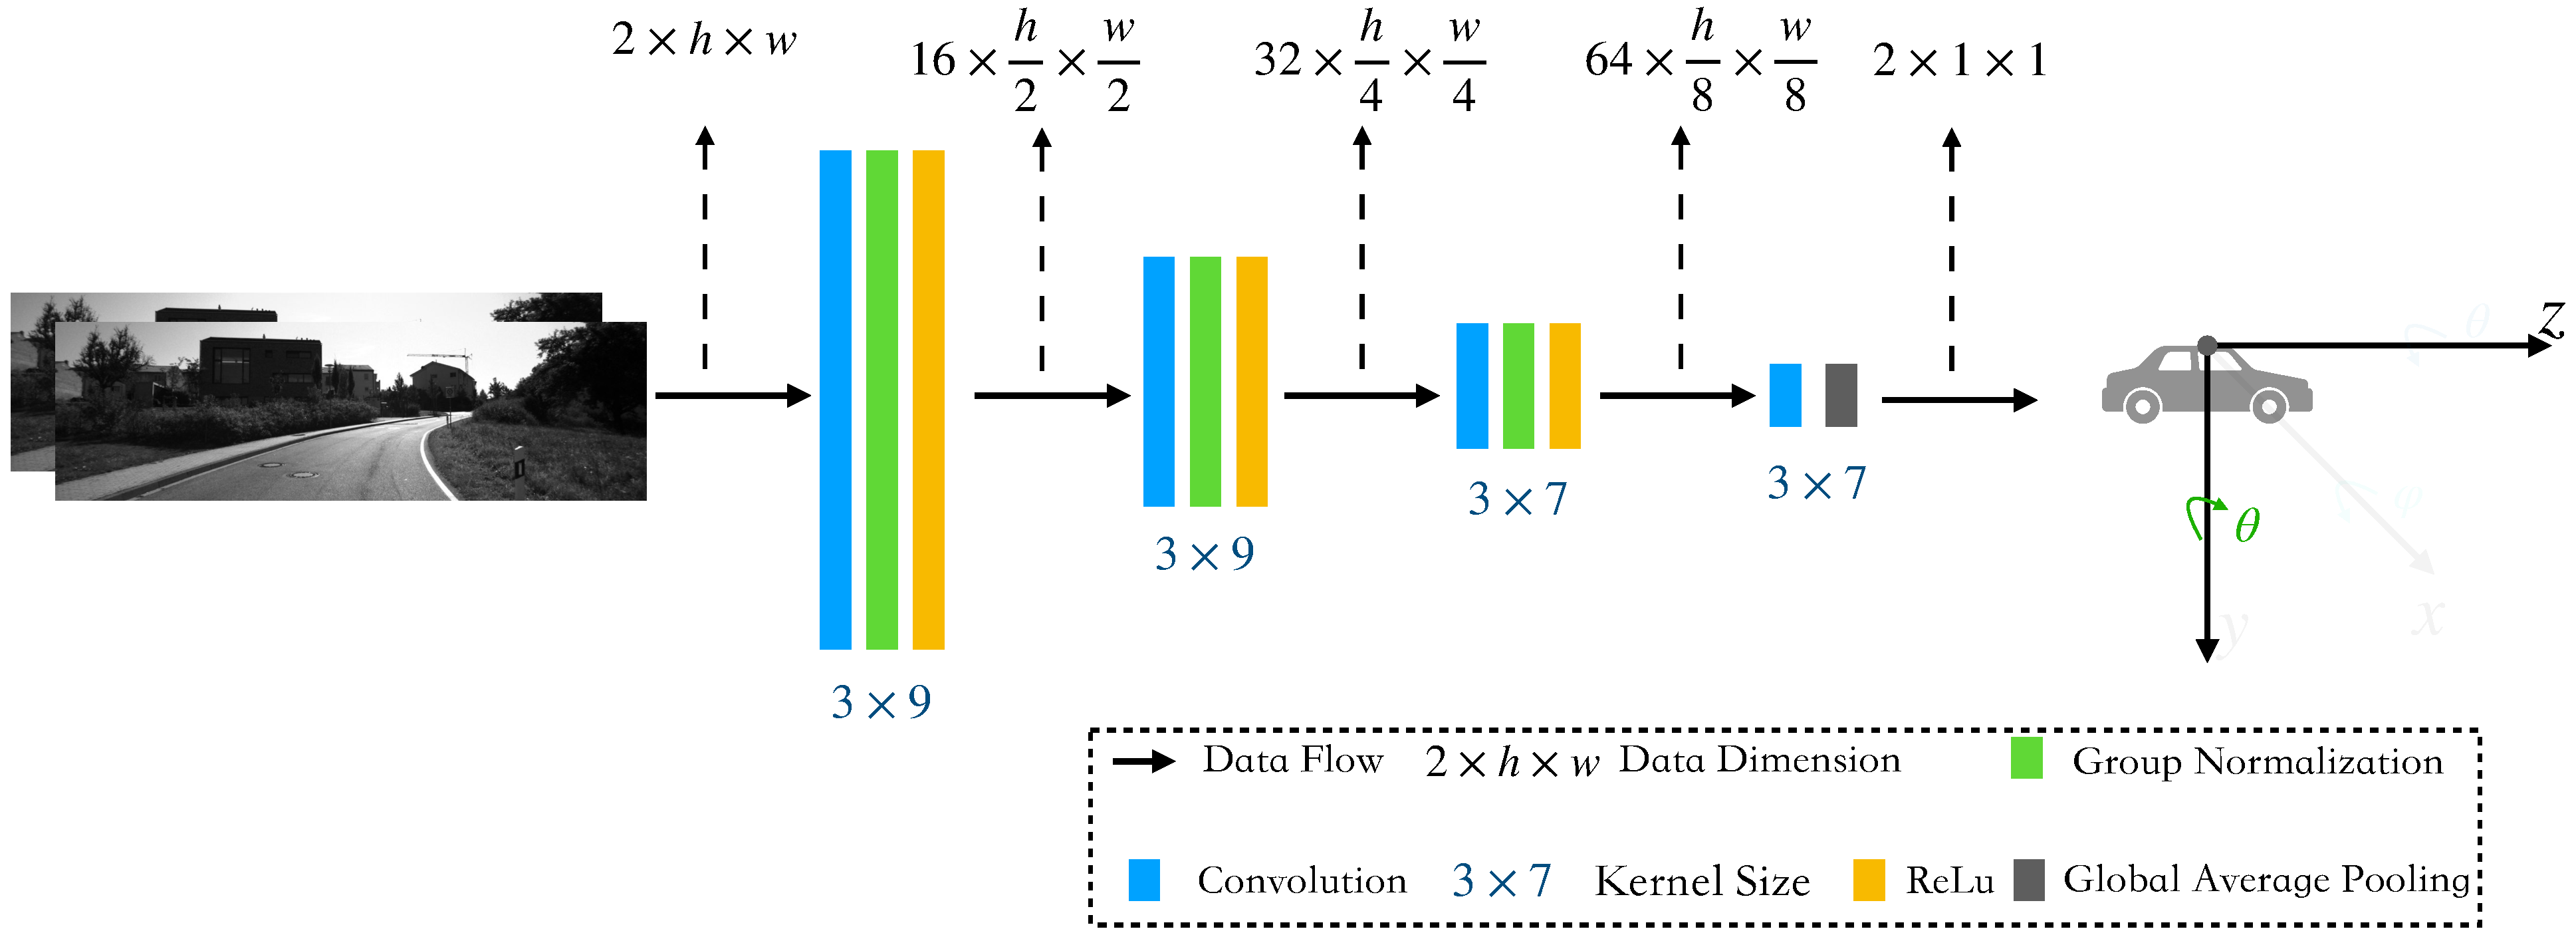
\includegraphics[width=0.95\textwidth]{datavo/network_structure_2-crop.pdf}
    \caption{轻量化网络架构结构图}
    \label{fig:nerwork_structure}
\end{figure}

本章构建了一个轻量化的网络来学习路面车辆的主要运动,网络架构如图\ref{fig:nerwork_structure}所示。
网络主要由卷积层构成,除最后一个卷积层以外,每个卷积后面都附加一个批归一化层(Batch Normalization) \cite{wu2018group} 和修正线性单元层(ReLU)。
同Zhou等人 \cite{zhou2017unsupervised}的架构一样,网络的最后一层没有使用全连接层,而是使用全局均值池化层\cite{lin2013network},
用以降低参数量,增强泛化性。此外,由于车辆运动引发的图像光流大部分为水平方向,尤其是在车辆旋转的情况下,如图\ref{fig:optical_flow}所示。
所以网络没有使用正方形的卷积核,而是通过使用宽大于高的卷积核来扩大水平方向的感受野。同时,本章使用了膨胀卷积(Dilated Convolution) \cite{yu2015multi},进一步在参数量相同的情况下扩大感受野。

\begin{figure}[ht]
    \centering
    \begin{subfigure}[b]{0.48\textwidth}
        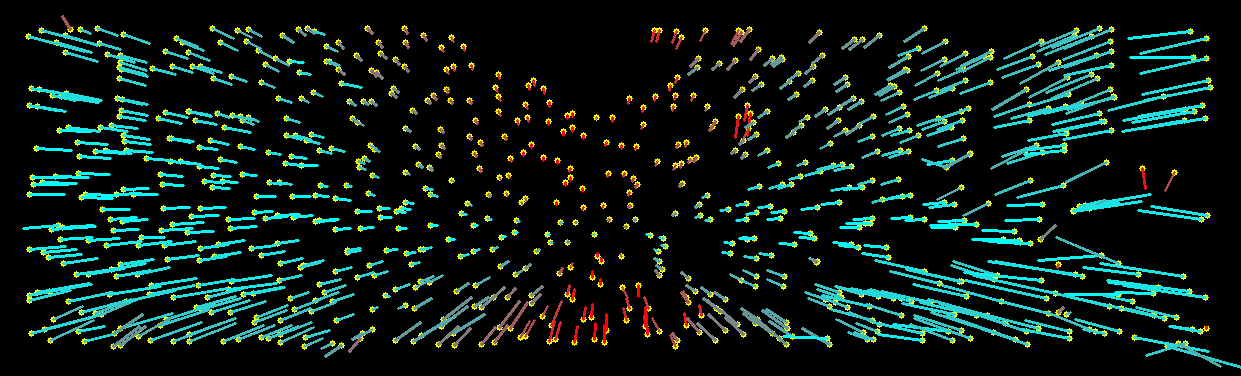
\includegraphics[width=\textwidth]{datavo/flow_61.png}
        \caption{车辆前行}
        \label{fig:optical_flow_f} 
    \end{subfigure}
    \vspace*{2mm}
    \begin{subfigure}[b]{0.48\textwidth}
        \includegraphics[width=\textwidth]{datavo/flow_52.png}
        \caption{车辆后退}
        \label{fig:optical_flow_b} 
    \end{subfigure}
    \vspace*{2mm}
    \begin{subfigure}[b]{0.48\textwidth}
        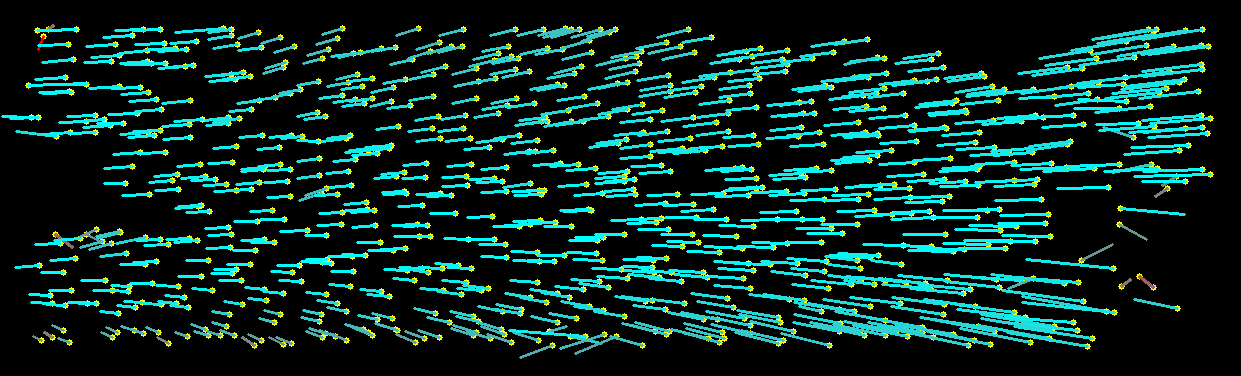
\includegraphics[width=\textwidth]{datavo/flow_196.png}
        \caption{车辆向左侧旋转}
        \label{fig:optical_flow_l} 
    \end{subfigure}
    \begin{subfigure}[b]{0.48\textwidth}
        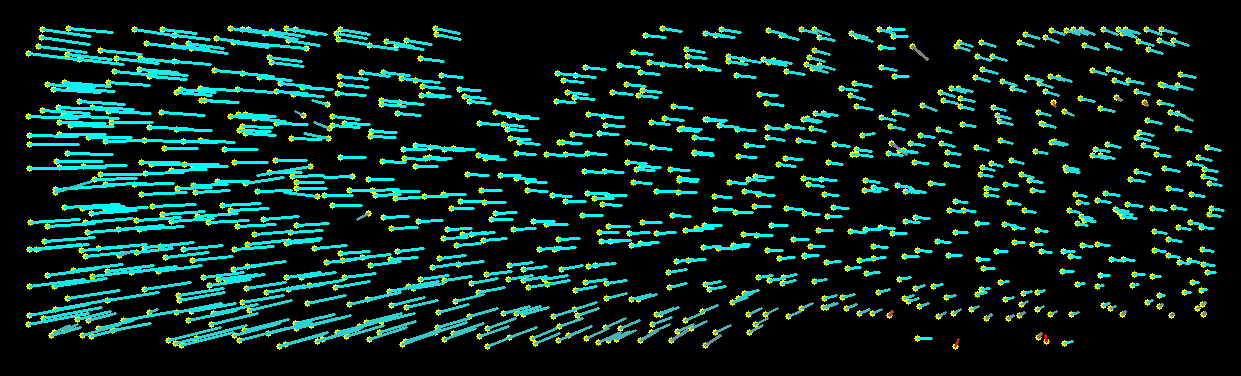
\includegraphics[width=\textwidth]{datavo/flow_96.png}
        \caption{车辆向右侧旋转}
        \label{fig:optical_flow_r} 
    \end{subfigure}
    \caption{路面车辆运动时的光流分析}
    \label{fig:optical_flow}
\end{figure}
模型的输入为由灰度图像叠加而成图像对,本章不仅使用相邻帧图像组合成的图像对(图像间隔为0)对作为输入,而是随机生成闭区间[-4,4]之间的一个整数,然后使用这个数作为图像对中两个图像之间的间隔,当做一个数据增加的手段。
模型的输出为与图像对对应的相机运动,表示为$Y$轴旋转运动$\theta $和前进运动$z'$。其中$Y$轴旋转运动$\theta$为旋转矩阵计算得来的欧拉角所对应的$Y$轴分量;
前进运动$z'$可使用公式\eqref{eq:decouple_z}计算。本章使用L2距离作为损失函数:
\begin{equation}
    L_2 = \|\underline{\theta} -\theta_p\|_2 +\|\underline{z} -z_p \|_2
\end{equation}
其中$\theta_p$和$z_p$为模型估计出的运动,$\underline{\theta}$和$\underline{z}$运动的真值。
本章使用ADAM优化器\cite{kingma2014adam}最小化损失函数获取模型参数,初始学习率设置为0.001,在第50个周期之后,学习率线性衰减,至100个周期衰减为0.0006。

模型训练成功之后,模型输入连续图像后可以得到与之对应的机器人旋转角 $\theta$前进距离$Z$。
首先根据公式\eqref{eq:r_t_ratio}计算平移偏角$\alpha$,并假设其它维度旋转均为0,然后构建旋转矩阵
$\mathbf{R}_\theta$和$\mathbf{R}_\alpha$,车辆的平移向量计算为$\mathbf{t}_\alpha = \mathbf{R}_\alpha (0,0,z)^T$。
运动矩阵可表示为:
\begin{equation}
    \mathbf{T}_i =\begin{pmatrix} \mathbf{R}_\theta & \mathbf{t}_\alpha\\ 0 & 1  \end{pmatrix} 
    \label{eq:rt_final}
\end{equation}
车辆的位姿可以通过运动矩阵的累积获取:
\begin{equation}
    \mathbf{P}_i = \mathbf{P}_{i-1}\mathbf{T}_i
    \label{eq:pose}
\end{equation}

\section{路面车辆模型实验}
\label{sec:datavo_experiments}
我们在公开数据集KITTI的视觉里程计数据\cite{geiger2012kitti}上对本章提出的算法进行评测和分析,使用其提供评价标准定量测量相对位姿误差(RPE),包括相对平移误差和相对姿态误差\cite{geiger2012kitti}。

本章算法使用Python程序语言实现,基于深度学习框架PyTorch进行网络模型搭建和模型训练,目前本章算法已经开源\footnote{https://github.com/TimingSpace/DMVOGV}。本章算法在一台具备16GB内存、因特尔Core i7(Intel i7-7700 CPU @ 2.80GHz )、英伟达GPU(GeForce GTX 1060)的笔记本电脑上进行测试。测试系统配备CUDA10.0,Python 3.6.9的Ubuntu操作系统。
由于所提出模型的轻量化,当训练批大小(Batch Size)为30时,模型训练仅需要2G的显存;在预测时,本章算法可以在CPU上达到200帧每秒的实时效果。

\subsection{实验结果}
我们首先评价运动聚焦引发的位置偏移;然后评价运动解耦对位置偏移的抑制效果;之后评价运动聚焦和解耦以及本章的轻量化网络架构带来的算法性能提升;最后与其它算法进行比较。

\subsubsection{运动聚焦造成的运动偏移的定量评测}
\label{sec:info_loss}
由于车辆运动受其机械结构和动力模型的约束,车辆主要运动集中于$Z$轴上的平移运动和$Y$轴上的旋转运动。此实验将定量分析在去除其它部分和全部维度的次要运动后,车辆位姿的偏移。
在具体实现上,首先忽略次要运动,然后重构机器人轨迹,并使用相对位置误差评价重构后的轨迹与原始估计之间的差异。在KITTI序列00至序列10上的相对位置误差的平均值记录于表\ref{tab:info_loss_1},并可视化于图\ref{fig:info_loss}中。
\begin{table}[h]
    \caption{Average RPE When Only Keeping Part of Vehicle Motion}
    \label{tab:info_loss_1}
    \begin{center}
    \begin{tabular}{c c c c c}
    \toprule
    % \hline
    \multirow{2}*{R / t} &{z}&{c}{xz}&{yz}&{zyz}\\
    & RPE(\%) /NID& RPE(\%) /NID& RPE(\%) /NID& RPE(\%) /NID\\
    %  % \hline%\hline
    \midrule
     y   &2.20  /4 & 2.06 /3 & 2.45 /3 & 2.34 /2 \\
     xy  &1.92  /3 & 1.77 /2 & 1.76 /2 & 1.56 /1 \\
     zy  &2.05  /3 & 1.91 /2 & 1.47 /2 & 1.27 /1 \\
     xyz &1.92  /2 & 1.81 /1 & 0.49 /1 & 0    /0   \\
    % \hline
    \bottomrule
    \end{tabular}
    \end{center}
 \end{table}
 \iffalse
 \begin{table}[t]
    \caption{Information Loss by Focusing only on translation along $z$ and roation about $y$}
    \label{tab:info_loss_2}
    \begin{center}
    \begin{tabular}{c c c c c c c c c c c c }
    \toprule
    % \hline
    seq & 00 & 01 & 02 & 03 & 04 & 05 & 06 & 07 & 08 & 09 & 10\\
    %  % \hline%\hline
    \midrule
     RPE(\%) &1.31 & 1.93 & 3.05 & 2.80& 2.22&1.30&1.34&1.19&1.44&3.79&3.85 \\
     ATE(m) &1.31 & 1.93 & 3.05 & 2.80& 2.22&1.30&1.34&1.19&1.44&3.79&3.85 \\
    % \hline
    \bottomrule
    \end{tabular}
    \end{center}
 \end{table}
\fi
\begin{figure}[ht]
    \centering
    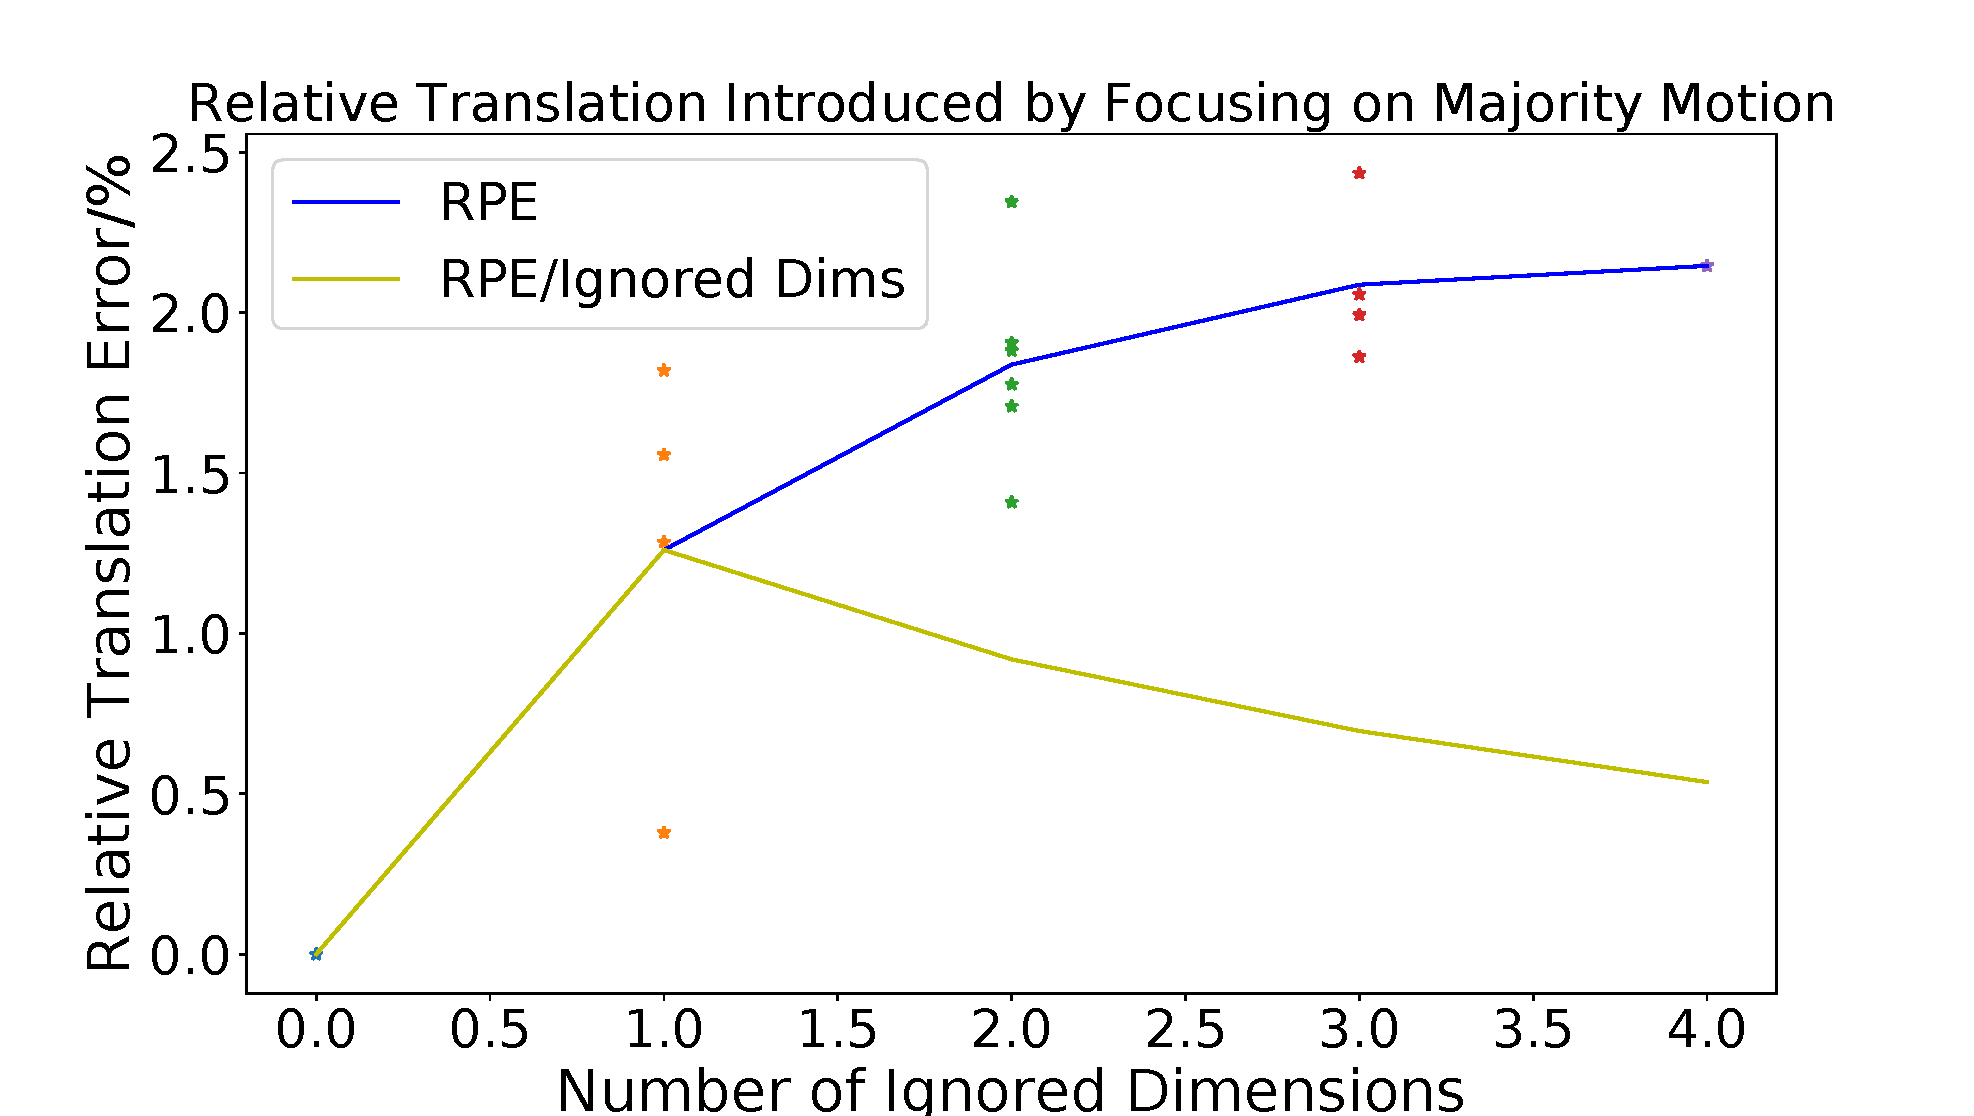
\includegraphics[width=0.95\textwidth]{datavo/info_loss.pdf}
    \caption{运动聚焦位置偏移可视化图}
    \label{fig:info_loss}
\end{figure}
表\ref{tab:info_loss_1}中,每一行保留着相同的旋转运动维度,每一列保留着相同的平移运动维度。 当仅保留$Y$轴旋转运动和$Z$轴平移运动(第一行第一列)时,平均位置误差为2.20\%。部分重构的轨迹可视化于图\ref{fig:path_recon},可见运动简化后的轨迹在水平面上依然与真实轨迹较为接近,但在竖直方向会因不同序列的高度变化产生不同的偏差(附录B中可视化了更多的重构轨迹)。

\begin{figure}[ht]
    \centering
    \begin{subfigure}[b]{0.48\textwidth}
    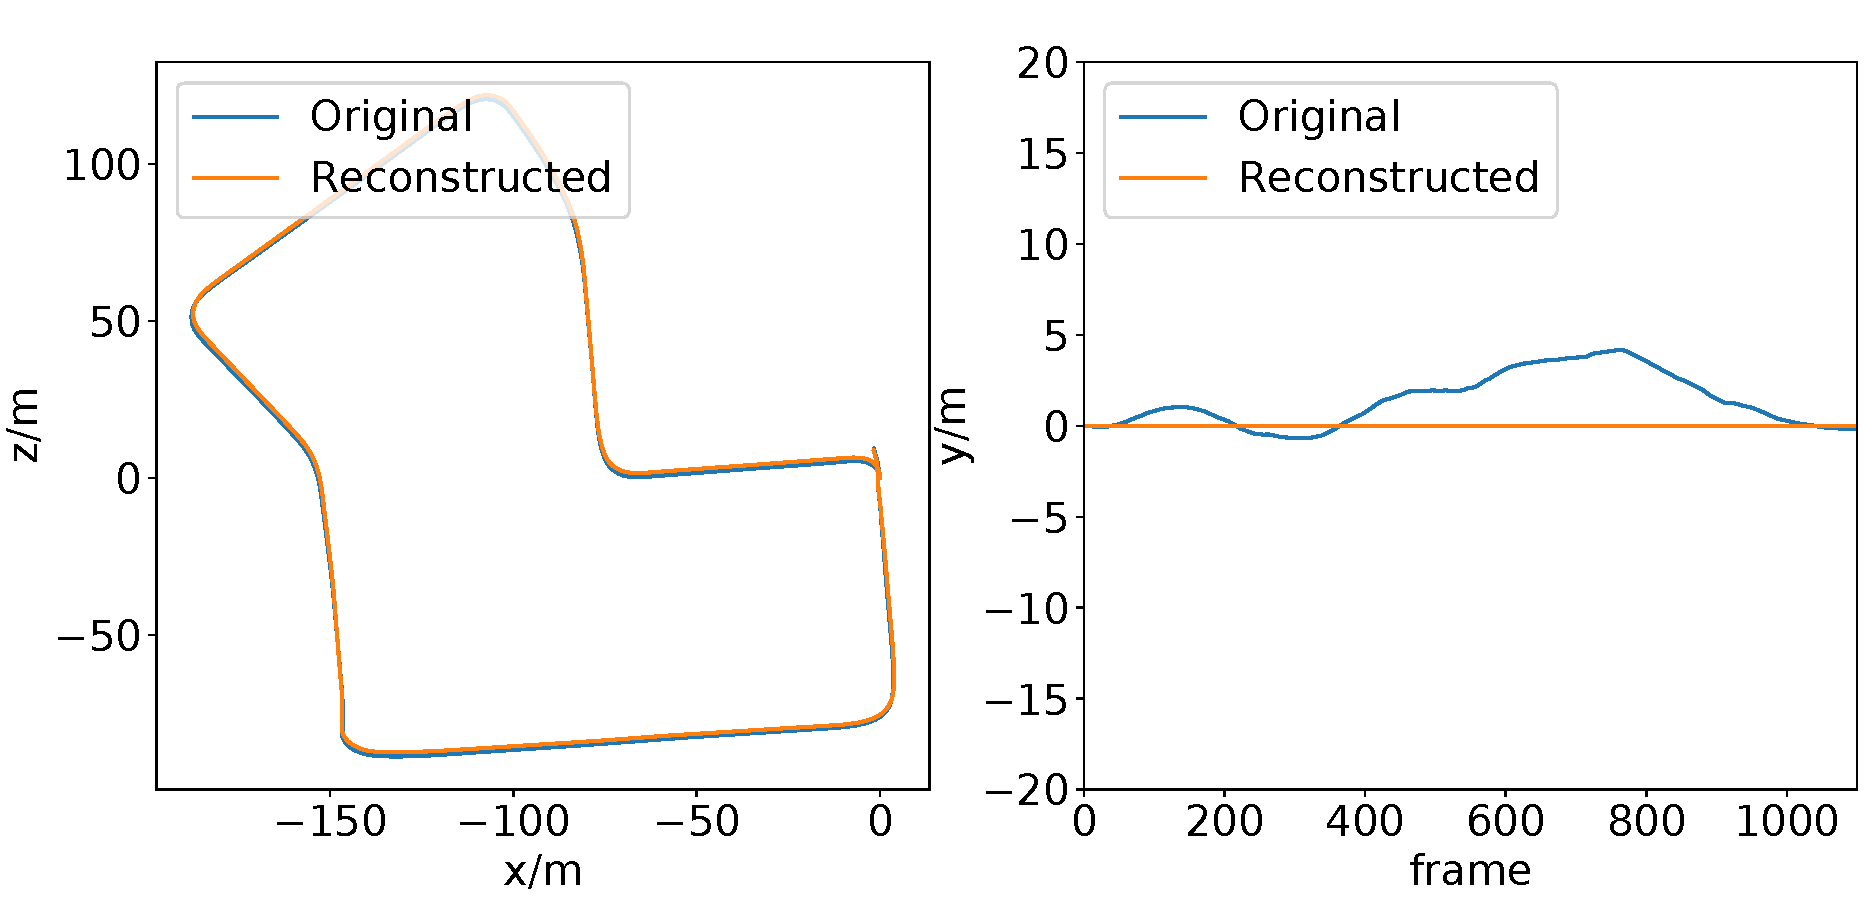
\includegraphics[width=\textwidth]{datavo/path_recon_07.pdf}
    \caption{KITTI 07}
    \label{fig:recon_07}
    \end{subfigure}
    \begin{subfigure}[b]{0.48\textwidth}
        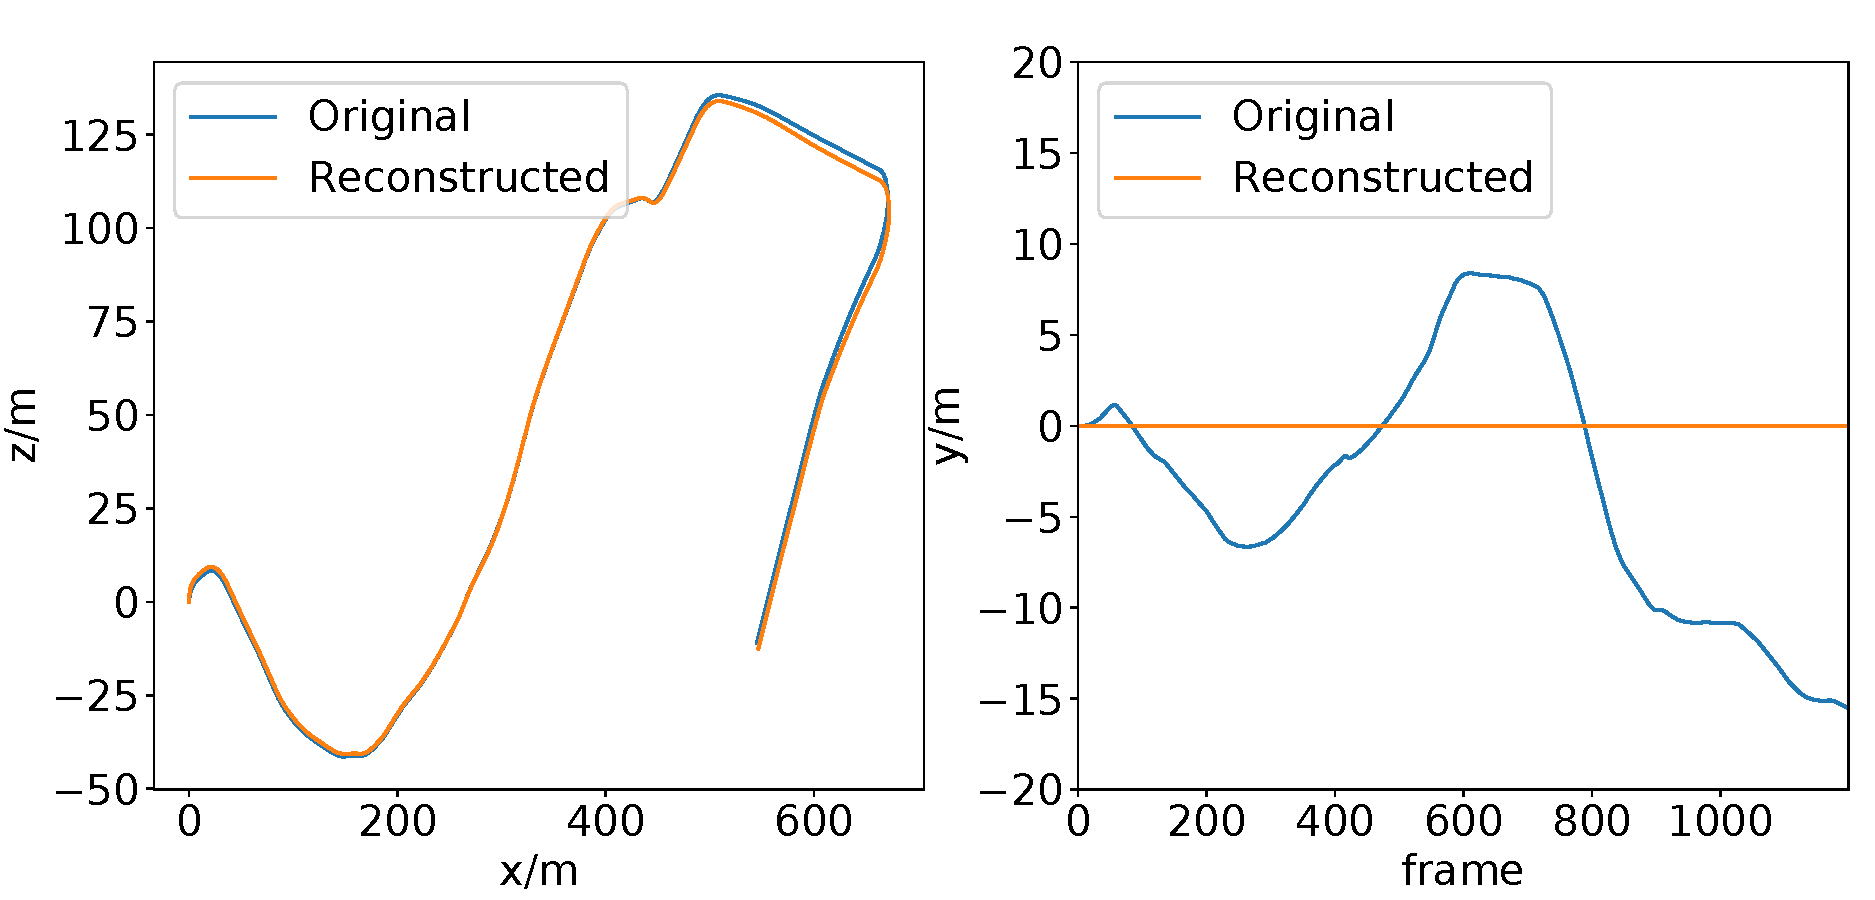
\includegraphics[width=\textwidth]{datavo/path_recon_10.pdf}
        \caption{KITTI 10}
        \label{fig:recon_10}
    \end{subfigure}
    \caption{运动聚焦后的轨迹重构图} 
    \label{fig:path_recon}
\end{figure}
我们将平均位姿误差(损失)与忽略维度的数量(增益)求商,如\ref{fig:info_loss}中的黄色线所示。这里比例系数可以作为一个相对平均损失。可见在仅保留$Z$轴平移运动和$Y$轴旋转运动时,相对损失比较小。


\subsubsection{运动解耦评测}
\label{sec:info_decouple}
本节将评价运动解耦对位姿偏移的矫正效果。根据公式\eqref{eq:r_t_ratio},车辆的平移偏角$\alpha$和车辆的旋转角$\theta$为线性关系。然而,其比例系数依赖于动态的车辆前进距离$z'$,并不是固定不变的。
首先研究使用静态的比例系数(即将比例系数设为固定值)的实验效果。我们使用不同的比例系数计算车辆偏移角,然后重映射车辆运动,得到的车辆评价位置误差可视化于图\ref{fig:static_decouple}。从图中可以看出,当比例系数为1.7时,评价误差最小,说明旋转时车辆的运动距离约为$\frac{1.7-0.5}{l}$米。为了更好的理解图中不同比例系数的物理意义,图中使用了不同颜色标出几个特殊的比例系数。红色图表示比例系数为0,此时平移运动不做任何映射,为原始的运动表示;比例系数为1时,认为平移偏角和旋转角度相同,根据公式\eqref{eq:frlt}的朴素映射解耦;黑色表示平移偏角为旋转角度的一半,这种情况仅在相机安装在后轴中心时才成立,但相机距离后轴中心相比于车辆前进距离较小时,此系数也可近似成立。

\begin{figure}[ht]
    \centering
    \begin{subfigure}[b]{0.48\textwidth}
        \centering
        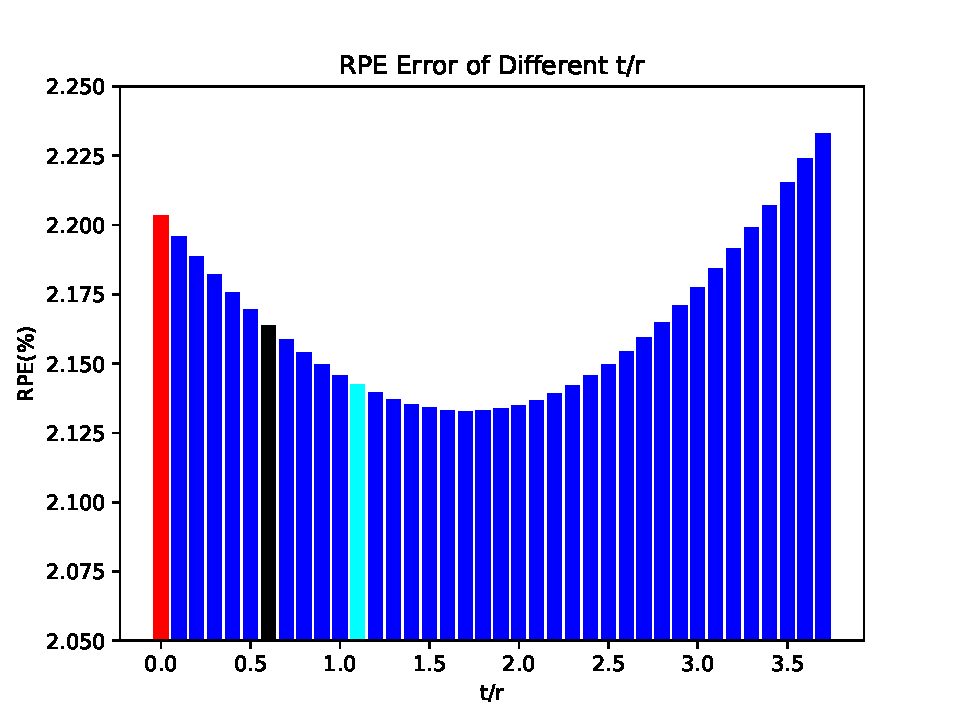
\includegraphics[width=\textwidth]{datavo/r_t_ratio.pdf}
        \caption{静态解耦}
        \label{fig:static_decouple}
    \end{subfigure}
    \begin{subfigure}[b]{0.48\textwidth}
        \centering
        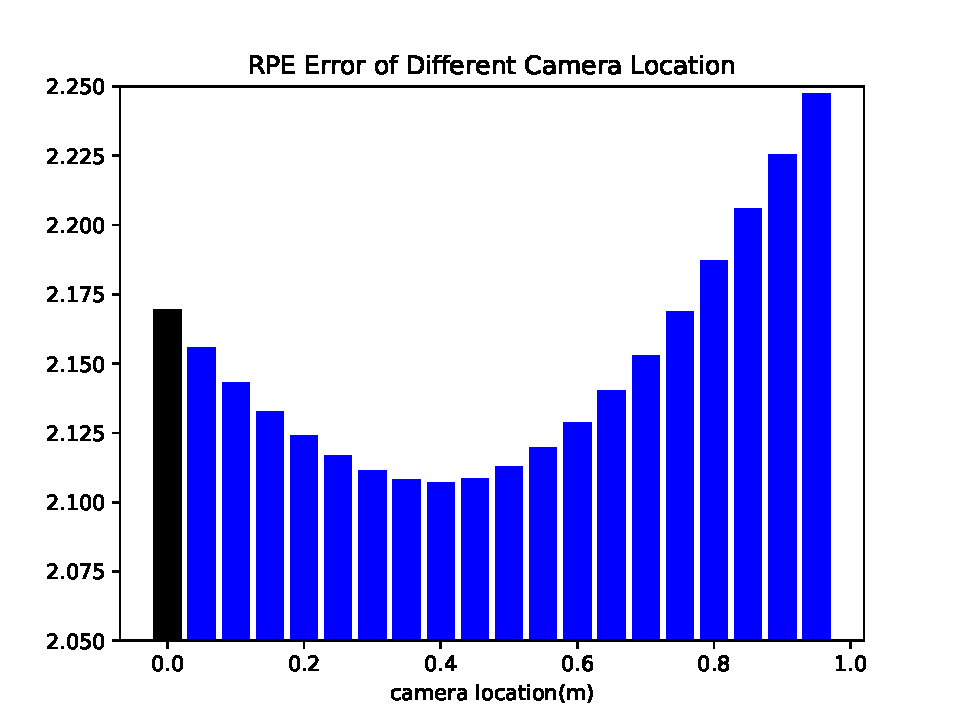
\includegraphics[width=\textwidth]{datavo/r_t_ratio_2.pdf}
        \caption{动态解耦}
        \label{fig:dynamic_decouple}
    \end{subfigure}
    \caption{运动解耦效果可视化}
    \label{fig:r_t_ratio}
\end{figure}

固定的比例系数无视了前进距离对平移偏角的影响,于是本节定量分析动态比例系数的位姿偏移。使用不同的相机偏距$l$,根据公式\eqref{eq:r_t_ratio},计算比例系数,然后求平均重构轨迹的相对位置误差,可视化于图 \ref{fig:dynamic_decouple},当相机偏距为0.4米时,重构误差最小。图中黑色为相机偏距为0时的重构误差,此时 $\alpha = 0.5 \theta$,和图\ref{fig:static_decouple}中的黑色物理意义相同,数值相等。

本节将动态映射和静态映射的效果进行了比较,记录于图\ref{fig:decouple}中。可以发现,两种运动解耦方式都降低了机器人轨迹的相对位置误差,动态解耦相比于静态解耦效果更好,更接近同时保留$X$轴平移和$Z$轴平移时的精度。

\begin{figure}[ht]
    \centering
    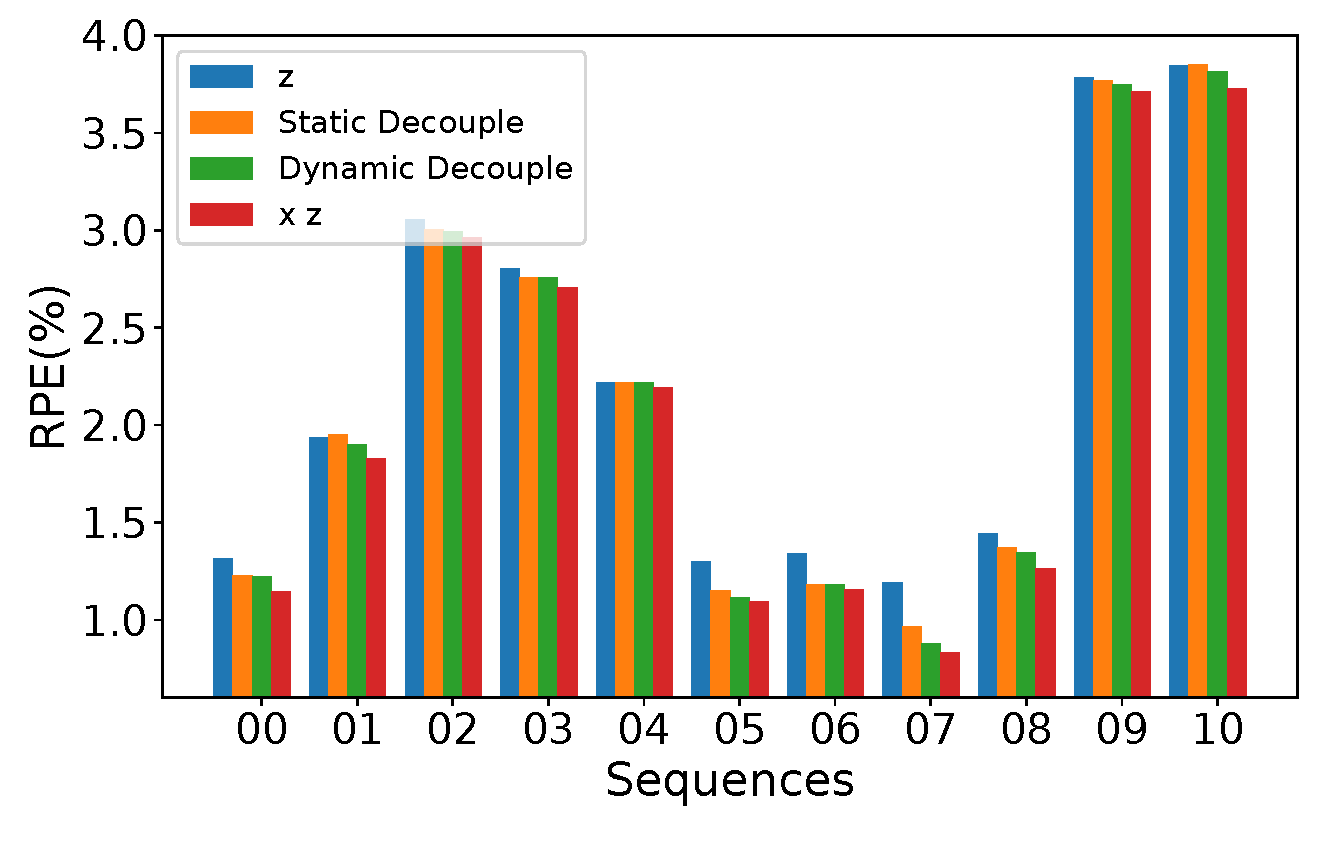
\includegraphics[width=0.95\textwidth]{datavo/decouple-crop.pdf}
    \caption{动态解耦和静态解耦效果对比图} 
    \label{fig:decouple}
\end{figure}

\subsubsection{运动简化的有效性验证}

\label{sec:ego_improvement}
\begin{table}[ht]
    \caption{The improvement of motion focusing}
    \label{tab:info_improve}
    \begin{center}
    \begin{tabular}{c c c c c c }
    \toprule
    % \hline
    \multirow{3}*{Train} & \multirow{3}*{Test} &\multicolumn{2}{c}{Learn All Motion} & \multicolumn{2}{c}{Learn $R_y, t_z$}\\
    & &Trans & Rot & Trans & Rot\\
    & & (\%) & (deg/m)  & (\%) & (deg/m)\\
    %  % \hline%\hline
    \midrule
     00 & 02 04 06 08 10 &26.8 & 0.137 & 23.9 & 0.110 \\
     00 02 & 04 06 08 10 &18.3 & 0.095 & 16.7 & 0.070 \\
     00 02 04 & 06 08 10 &17.6 & 0.091 & 16.9 & 0.076 \\
     00 02 04 06 & 08 10 &15.3 & 0.082 & 13.2 & 0.065   \\
    % \hline
    \bottomrule
    \end{tabular}
    \end{center}
 \end{table}

本节设计对比实验以证明运动聚焦和解耦的有效性。使用相同的训练数据训练如下两种模型:
1) 运动简化模型(Motion Focusing Model,MFM)仅学习车辆的前进运动和旋转运动;  2) 全运动模型 (All Motion Model,AMM), 学习车辆六个自由度
的全部运动。本节在多个训练和测试数据序列的组合上进行多次实验以减低随机性的影响。在实验过程中,我们记录了网络训练时的损失函数变化曲线和测试时的相对平移误差。
如图\ref{fig:training_loss}所示,运动简化模型收敛速度相比于全运动模型有着大幅提高。
\begin{figure}[ht]
    \centering
    \begin{subfigure}[c]{0.48\textwidth}
        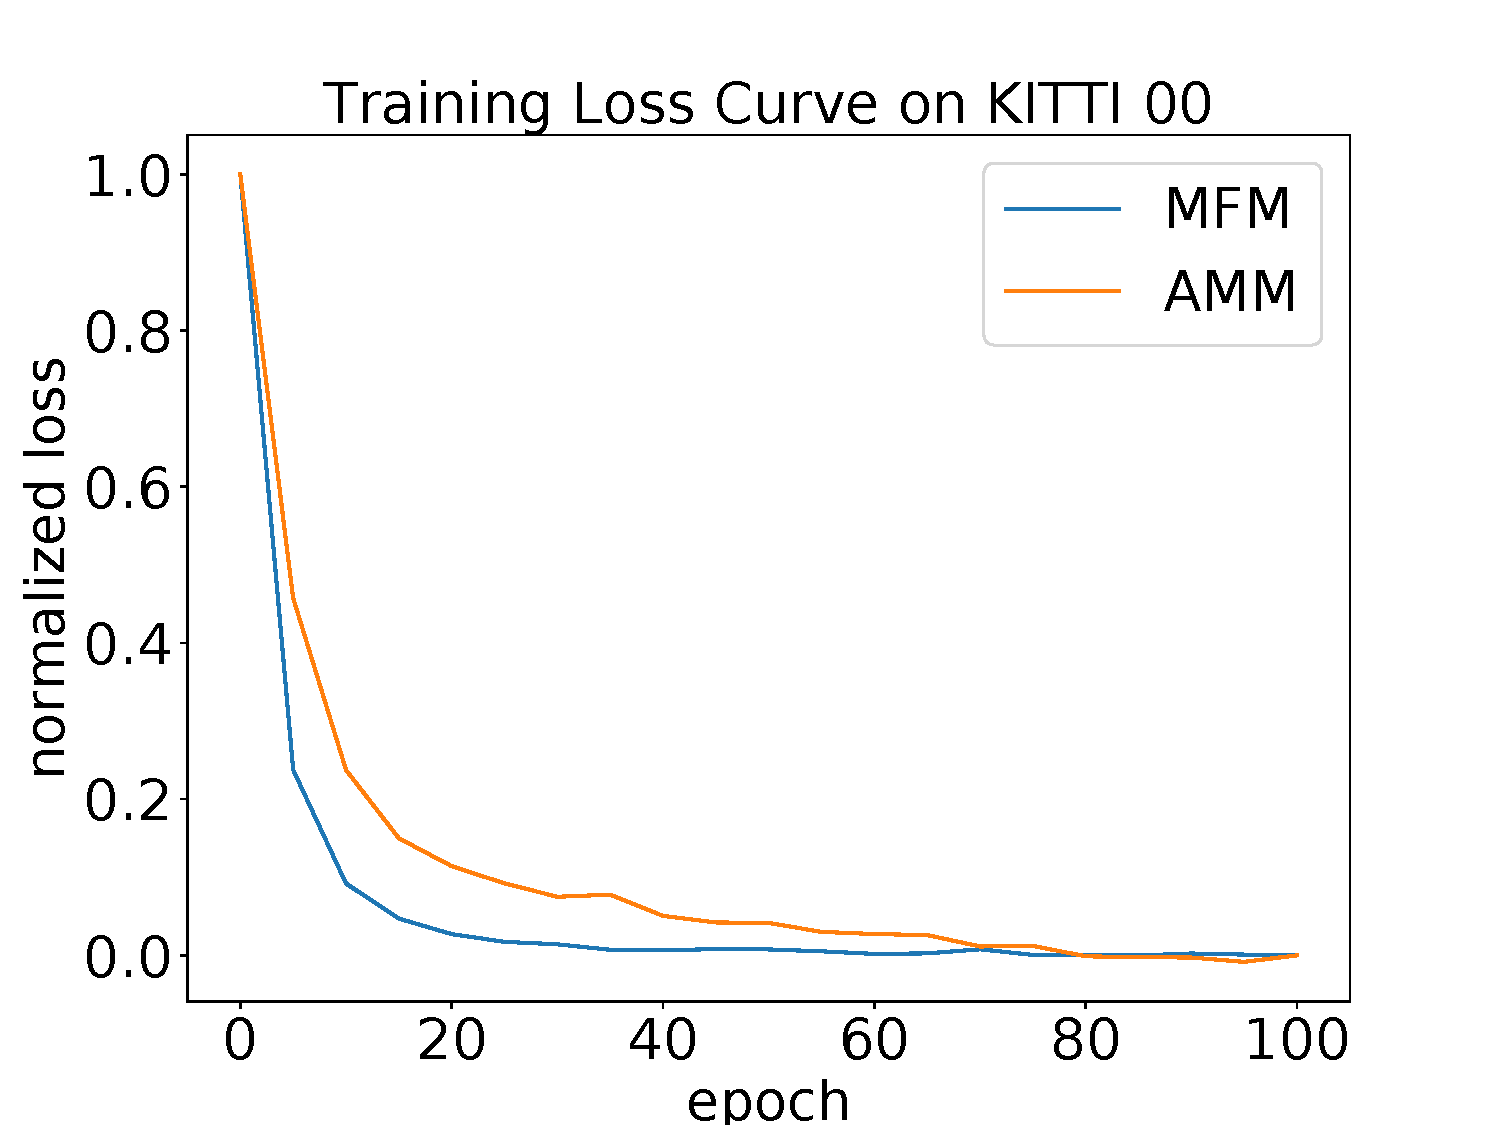
\includegraphics[width=\textwidth]{datavo/training_loss_0.pdf}
        \caption{00}
        \label{fig:tl_0}
    \end{subfigure}
    \vspace*{2mm}
    \begin{subfigure}[c]{0.48\textwidth}
        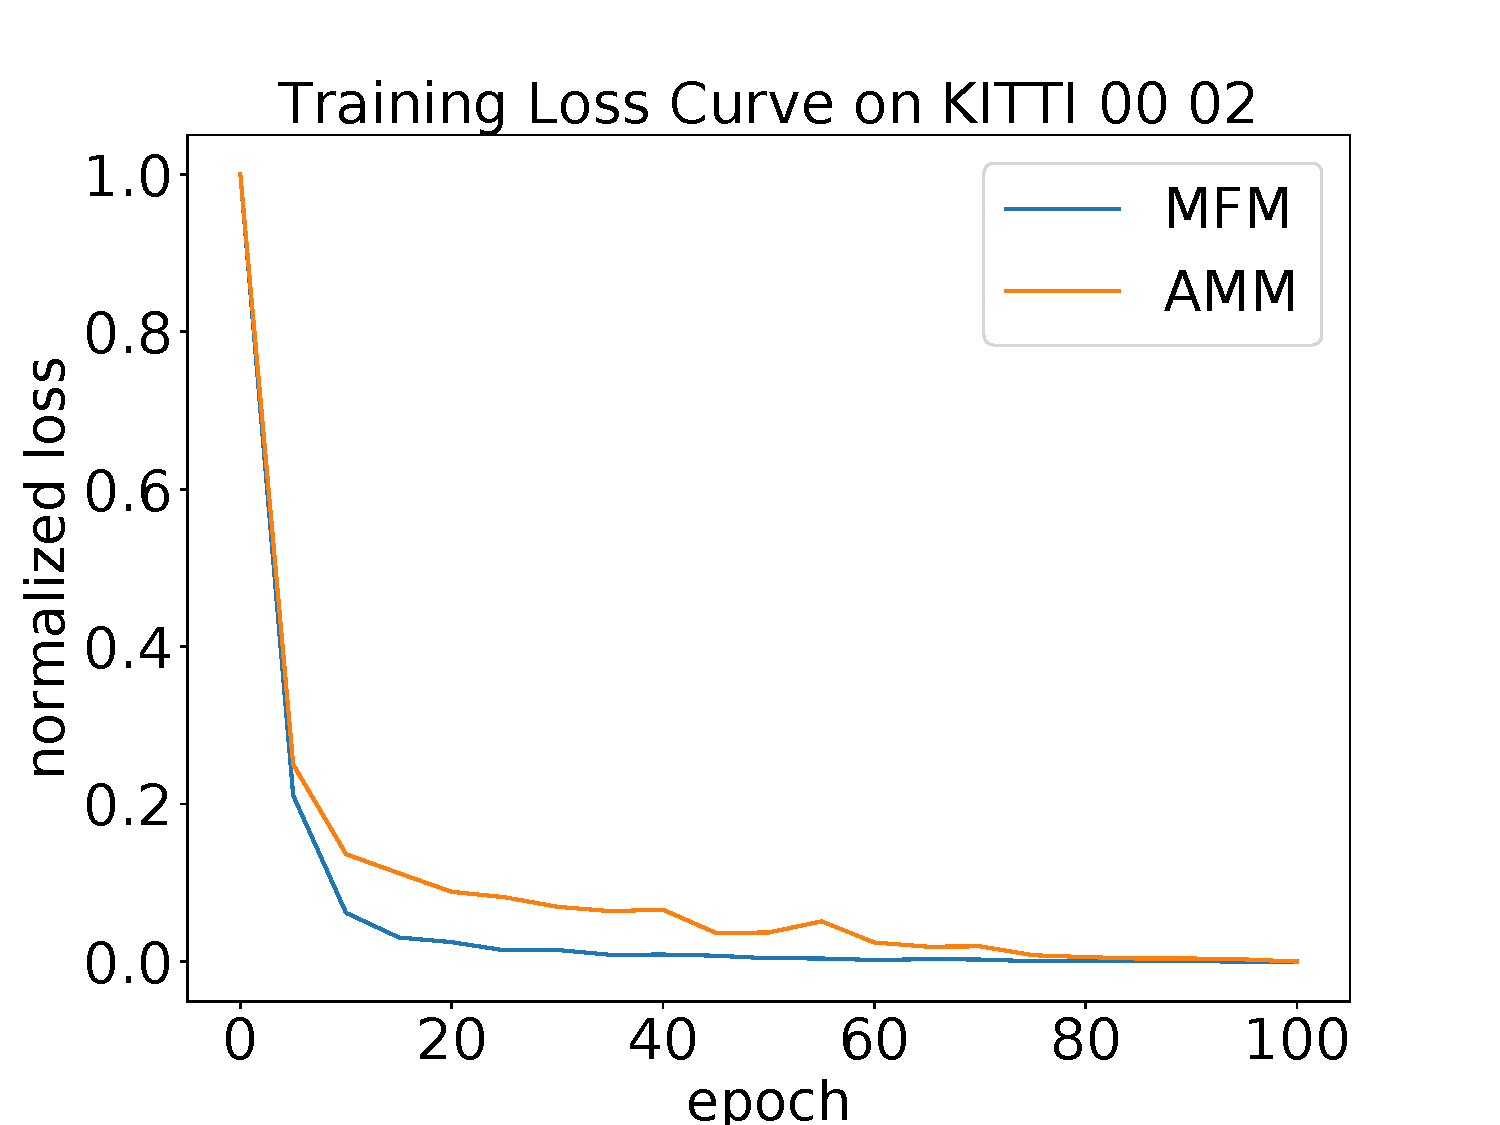
\includegraphics[width=\textwidth]{datavo/training_loss_0-2.pdf} 
        \caption{00-02}
        \label{fig:tl_02}
    \end{subfigure}
    \vspace*{2mm}
    \begin{subfigure}[c]{0.48\textwidth}
        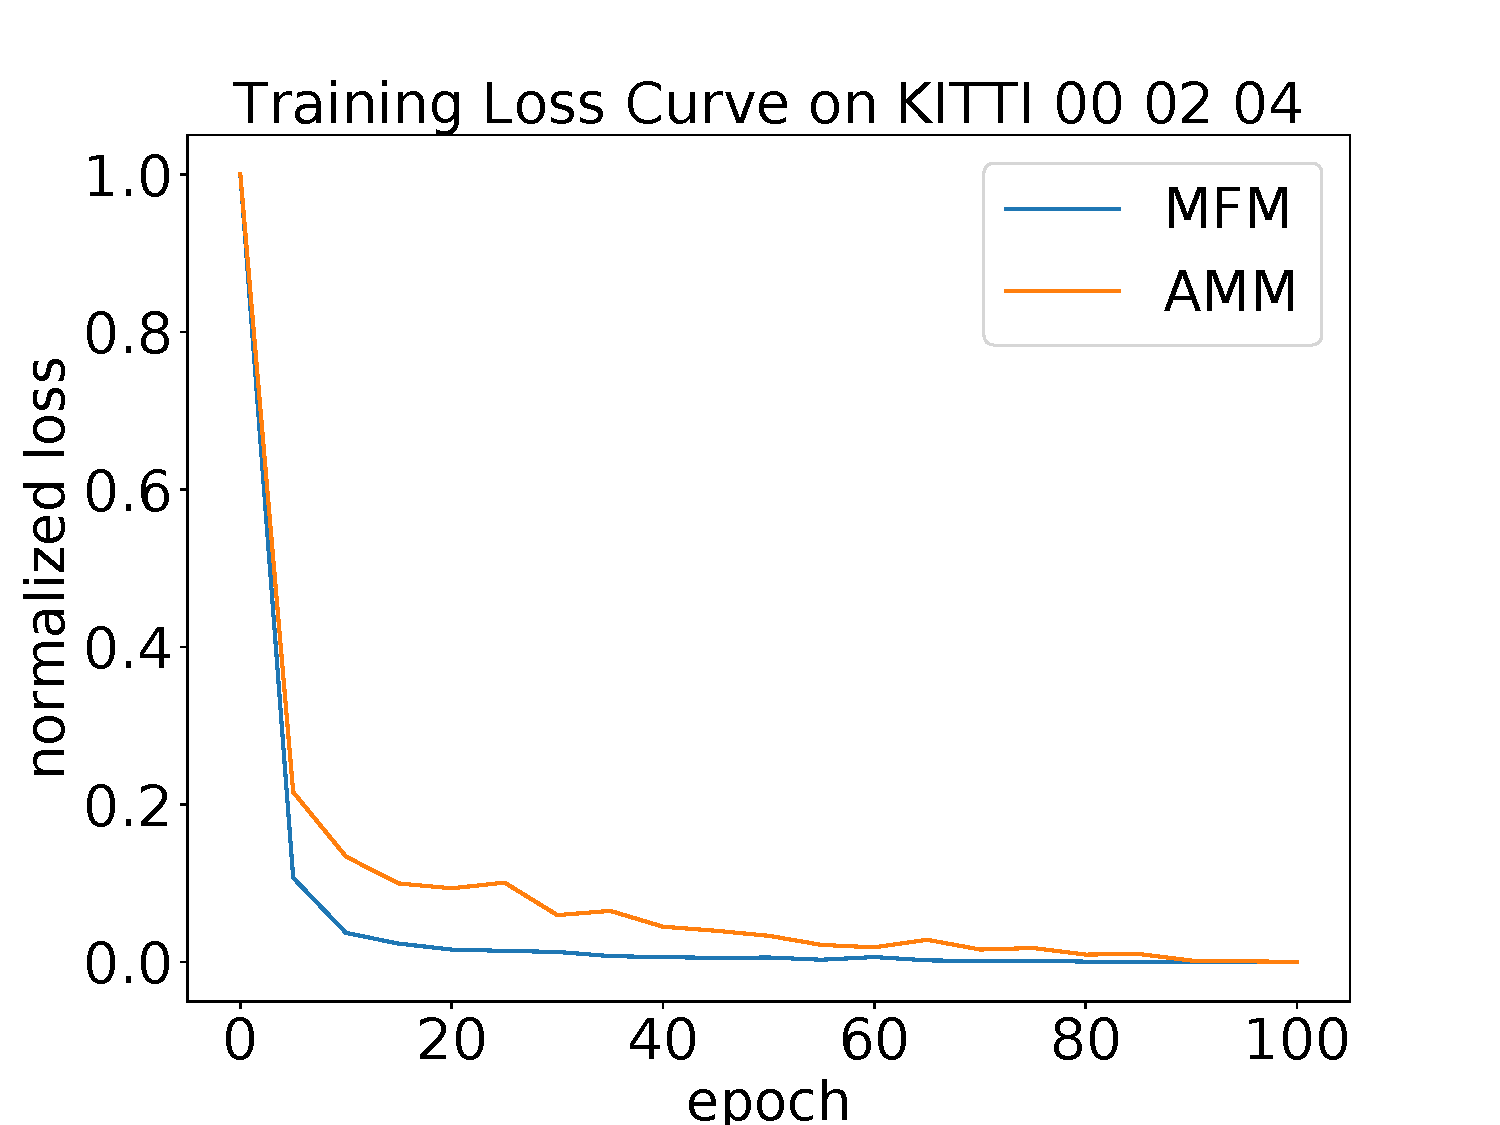
\includegraphics[width=\textwidth]{datavo/training_loss_0-4.pdf} 
        \caption{00-04}
        \label{fig:tl_024}
    \end{subfigure}
    \begin{subfigure}[c]{0.48\textwidth}
        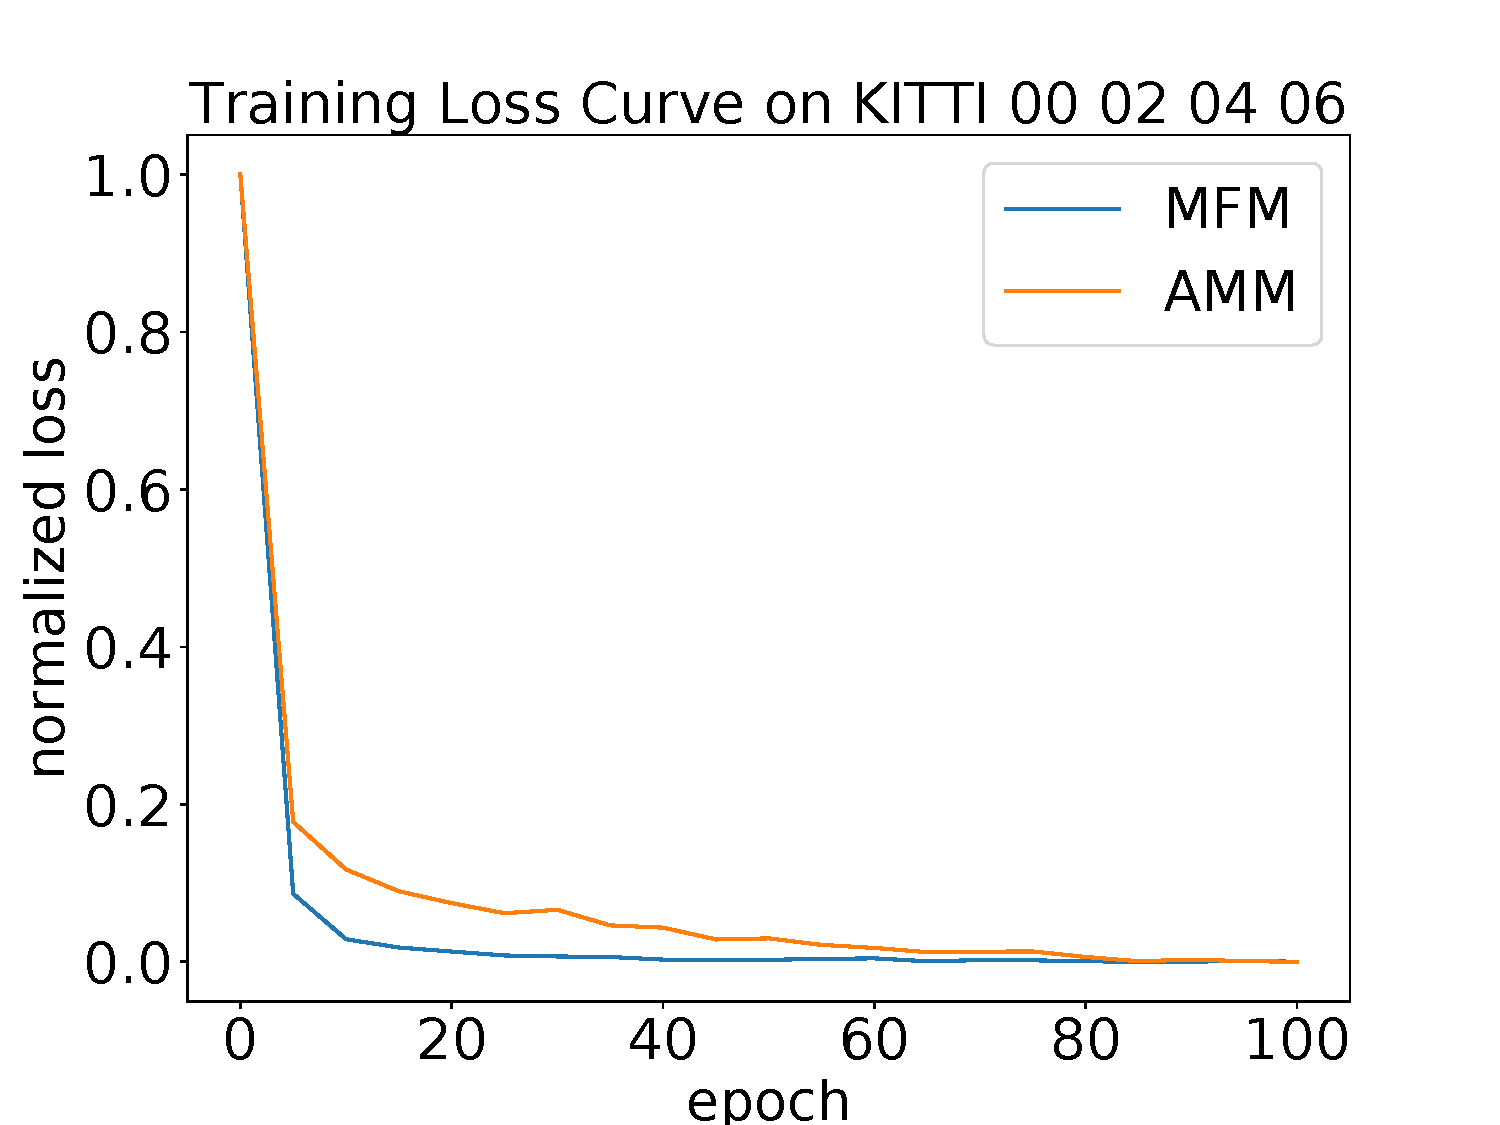
\includegraphics[width=\textwidth]{datavo/training_loss_0-6.pdf} 
        \caption{00-06}
        \label{fig:tl_0246}
    \end{subfigure}
    \caption{训练损失函数收敛速度对比图}
    {\label{fig:training_loss}}
\end{figure}

\begin{figure}[ht]
    \centering
    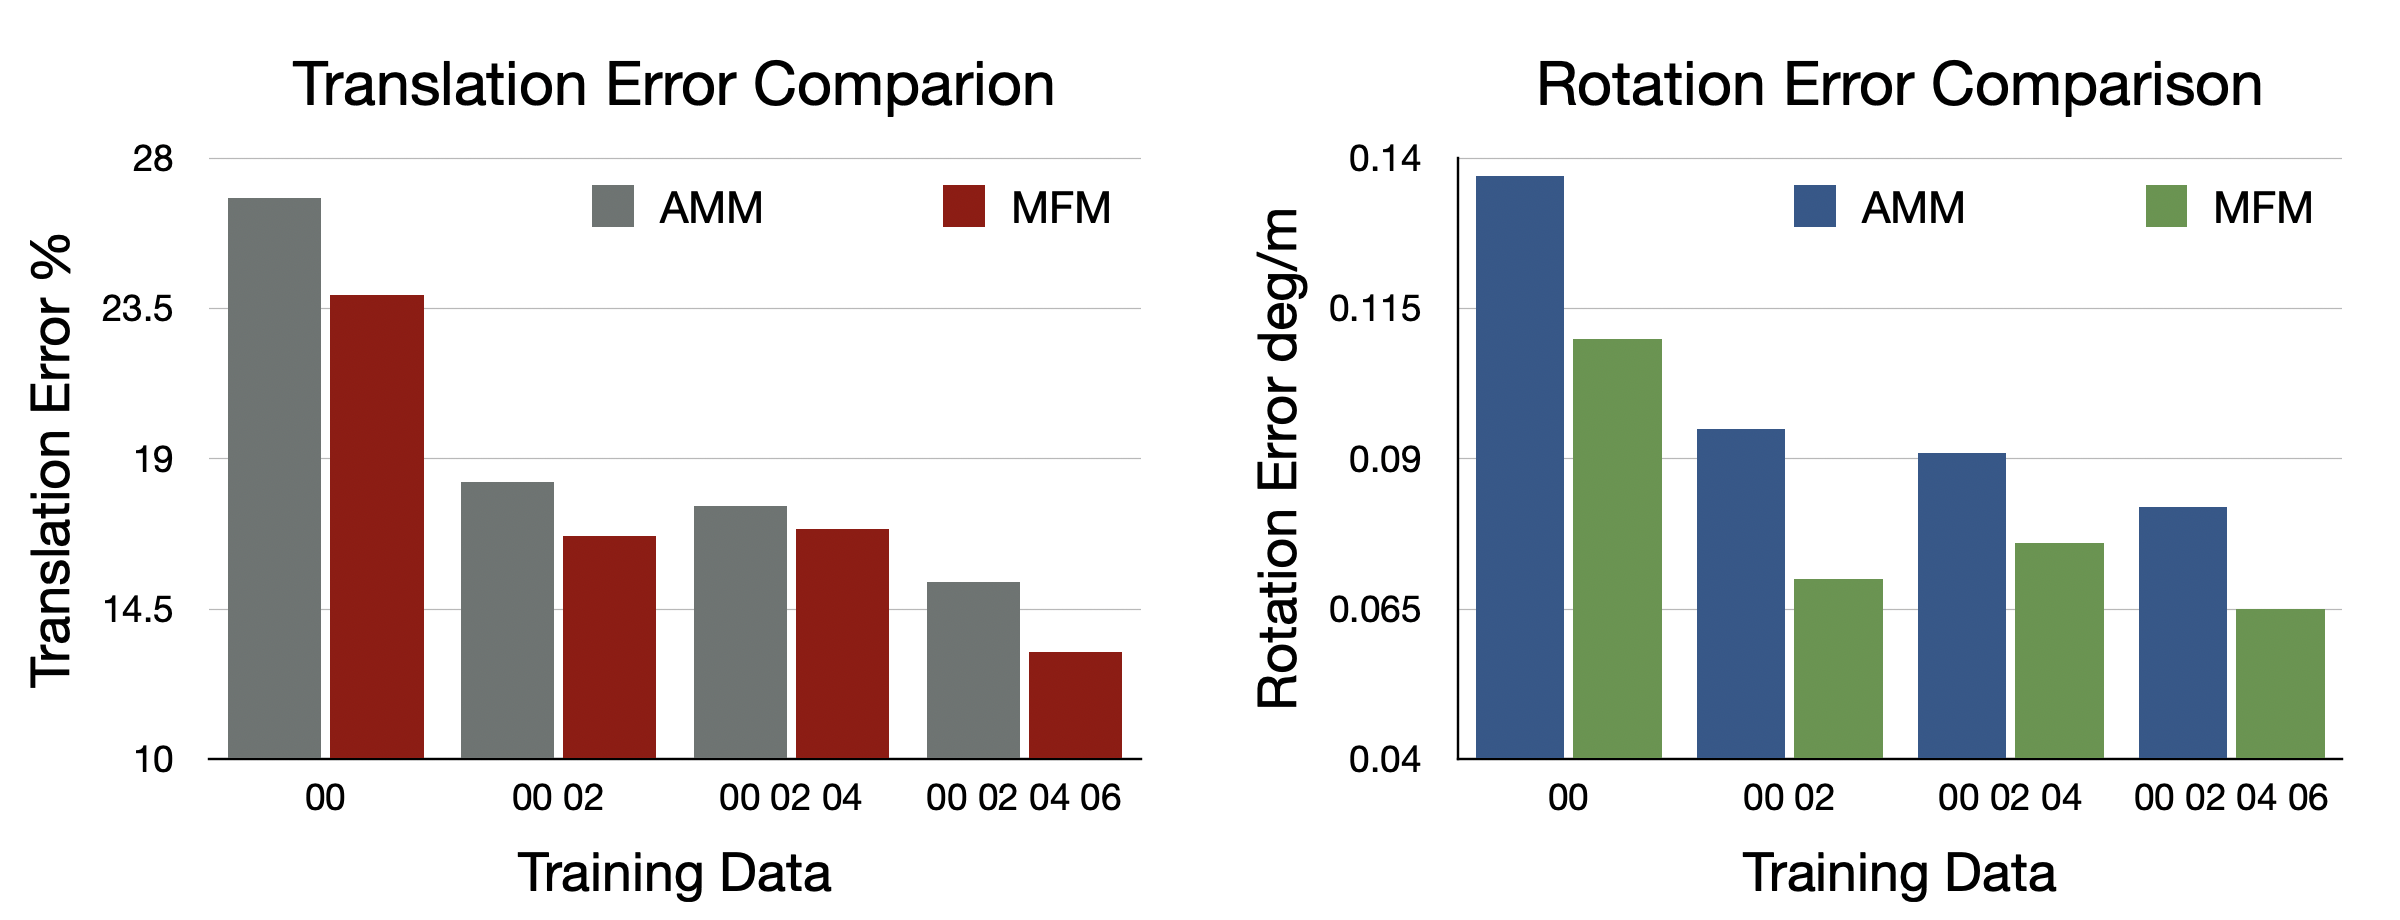
\includegraphics[width=0.95\textwidth]{datavo/focusing_train.png}
    \caption{运动聚焦与解耦前后效果对比图}
    \label{fig:focucing_train}
\end{figure}
不同训练模型的测试误差记录在表\ref{tab:info_improve},并可视化于图\ref{fig:focucing_train}。
可以看出,运动简化模型的测试精度相比于全运动模型在不同数据组合的情况下均有一定提高:其中相对平移误差提高约2\%,
相对姿态误差提高约每米0.2度。可见,尽管运动聚焦和运动解耦使训练目标轨迹与真实轨迹相比出现了一定的偏移,但整体来看,测试精度
仍然有所提升。另外,我们发现,无论是运动简化模型还是全运动模型,随着训练数据集数据量的不断增加,测试误差均不断降低。

\subsubsection{与其它算法比较}
\label{sec:compare}
\begin{table}[!htbp]
    \caption{与其他基于学习的视觉里程计方法比较结果}
    \begin{center}
    \begin{tabular}{c c c c c c c c c c c c c c}
    \toprule
    % \hline
    \multirow{4}*{Seq} & \multicolumn{2}{c}{Zhan et al.} &\multicolumn{2}{c}{DeepVO} & \multicolumn{2}{c}{SfM-Learner.}& \multicolumn{2}{c}{GeoNet}&  \multicolumn{2}{c}{\multirow{2}*{Our Method }}\\
                       & \multicolumn{2}{c}{(from \cite{zhan2018unsupervised})}  & \multicolumn{2}{c}{(from \cite{wang2017deepvo})}&\multicolumn{2}{c}{(from \cite{zhou2017unsupervised})} &\multicolumn{2}{c}{(from \cite{yin2018geonet})} &\\
    %  % \hline%\hline
    \cline{2-3}  \cline{4-5}  \cline{6-7} \cline{8-9} \cline{10-11} \cline{12-13}
        & Trans & Rot  & Trans & Rot  & Trans & Rot &Trans & Rot& Trans & Rot\\ 
    & (\%) & (deg/m)  & (\%) & (deg/m)  & (\%) & (deg/m)& (\%) & (deg/m) & (\%) & (deg/m) \\
    \midrule
        09&11.92&0.0360&-&-&17.84&0.0678&26.93&0.0954&9.26&0.0229 \\
        10&12.62&0.0343&8.11&0.0883&37.91&0.1778&24.69&0.0843&9.10&0.0221 \\
    \midrule
    % \textbf{Avg.} & \textbf{84.0}\\
    Avg & 12.27 & 0.0351 &8.11 &0.0883  & 28.88 &0.1228 &25.81& 0.0899& 9.18&\textbf{0.0225}\\
    % \hline
    \bottomrule
    \end{tabular}
    \end{center}
    \label{tab:data_kitti_compare}
    \end{table}
    
    \begin{table}[!htbp]
        \caption{与其他传统视觉里程计方法比较结果}
        \begin{center}
        \begin{tabular}{c c c c c c c c c c c c c c c c c c}
        \toprule
        % \hline
        \multirow{4}*{Seq} & \multicolumn{2}{c}{LIBVISO2} &  \multicolumn{2}{c}{ORBSLAM}& \multicolumn{2}{c}{\multirow{2}*{Our Method }}\\
                           &  \multicolumn{2}{c}{(from \cite{Song2015MoncularScale})}&\multicolumn{2}{c}{(from \cite{raul2015orb})}  &\\
        %  % \hline%\hline
        \cline{2-3}  \cline{4-5}  \cline{6-7} 
            & Trans & Rot  & Trans & Rot  & Trans & Rot\\ 
        & (\%) & (deg/m)  & (\%) & (deg/m)  & (\%) & (deg/m)& \\
        \midrule
            09&4.04& 0.0143&15.30&0.0026& 9.26&0.0229\\
            10&25.20 &0.0388&3.68&0.0048 &9.10&0.0221\\
        \midrule
        % \textbf{Avg.} & \textbf{84.0}\\
        Avg &14.62 & 0.0266& 9.49&0.0037 &\textbf{9.18}&0.0225\\
        % \hline
        \bottomrule
        \end{tabular}
        \end{center}
        \label{tab:data_kitti_compare_ge}
        \end{table}
    
我们将算法与其它基于学习的以及基于几何计算的方法进行定量比较。模型的训练集和测试集与其它基于卷积神经网络的方法\cite{zhan2018unsupervised,zhou2017unsupervised,yin2018geonet}一致:使用KITTI数据集00-08进行训练,在序列09和10上进行测试。
测试平均误差记录于表\ref{tab:data_kitti_compare}和表\ref{tab:data_kitti_compare_ge}中。

由于SfM-Learner\cite{zhou2017unsupervised}和GeoNet \cite{yin2018geonet}训练时并无绝对尺度信息,所以在评价其误差之前,先将其与真实轨迹进行了对齐。
ORB-SLAM\cite{raul2015orb}的单目版本和LIBVISO\cite{Geiger2011IV}的单目版本也需要与真实轨迹对齐。

从表\ref{tab:kitti_compare}中可以看出本章算法的效果优于只基于卷积神经网络的方法\cite{zhan2018unsupervised,zhou2017unsupervised,yin2018geonet} 与融合卷积神经网络和递归神经网络的DeepVO\cite{wang2017deepvo}精度不相上下。
和传统方法LibVISO2\cite{Geiger2011IV}和ORB-SLAM单目\cite{raul2015orb}相比,本章算法获取了更好的平均精度(见表\ref{tab:data_kitti_compare_ge})。

\subsection{实验结果讨论}
本节将依据实验数据对算法是否有效,算法为什么有效以及算法的局限性和解决方案等几个角度对实验结果进行讨论。
\subsubsection{算法有效性}
根据上述实验结果,可以从如下四个方面总结。
1)运动聚焦并不会引入过多的位姿偏移。运动聚焦之后,轨迹平均位置误差为2\%,其意味着在机器人运行100m后,其平均偏移量大概为2m。从可视化的重构轨迹中可以看出,这个偏移量相对很小。2)运动解耦可以进一步减少位姿偏移。运动解耦通过解耦$Y$轴旋转运行和$X$轴平移运动之间的耦合性,抑制了去除x平移后的位姿偏移,其中所提出的动态解耦算法优于静态解耦算法。在动态解耦算法中,相机到后轴的距离作为一个主要参数,本章实验中该距离为通过数据计算得到,在实际情况中也可以通过标定测量获取。3)运动聚焦和运动解耦提升了算法性能,主要体现在两个方面:运动聚焦和解耦之后的模型可以更快的收敛,普通模型需要大约60个训练周期,而优化后模型在20个训练周期之后即可收敛,收敛时间降为原来的三分之一;此外,运动聚焦和解耦之后的模型提升了运动估计的精度,在所有的对比实验中,性能都优于普通模型。4)与其它算法相比,我们取得更好的效果。在对比中可以发现,几何方法并不鲁棒,在不同测试集中效果差异较大,而本章算法取得了更好的平均效果;另外,我们的算法优于其它基于卷积神经网络的算法,但与借助递归神经网络的DeepVO基本持平,我们取得了更小的姿态误差,而DeepVO取得了更小的平移误差。

\subsubsection{算法有效性原因分析}
运动聚焦和运动解耦的有效性可以从三个角度解释:1)首先,由于地面车辆的运动受其自身机械结构和动力机制的约束,其不具备完善的三维空间内的6自由度运动模式,所以在不考虑非主要运动维度上的运动时,并不会造成过大的位置偏移,这一论点在第\ref{sec:info_loss}节得到验证,是本章方法的可行性基础;2)由于非主要维度的运动幅度非常小,导致其信噪比不高,尝试去学习这些维度的运动,会使神经网络模型容易被噪声干扰。3)由于本章算法仅学习两个主要维度,所学习目标变得相对简单,进而一个轻量级的模型就可以去学习拟合这个映射,这样数据也就相对充足,而充足的数据会提升算法的性能(如表 \ref{tab:info_improve})。

\subsubsection{算法局限性及解决方案}
当车辆的运动大部分局限在水平面上时,本章所提出的算法可以取得较好的效果,如果车辆有较多的$X$轴转动时,算法的精度会下降。如图 \ref{fig:decouple}所示,由于序列09和10存在较大比例的非水平运动,所以序列09和10的RPE误差也相对较大。为了解决这个限制,一种可行的方案为,使用其它传感器(如惯性传感器)测量车辆$X$轴的转动,作为本章算法的一个补充。

此外,本章假设视觉传感器水平朝前安装,但当相机的安装角度不是水平时,车辆的前进运动会被映射为前进分量和上下运动分量。在这种情况下,需要在初始阶段,标定相机与水平线的俯仰角$\sigma$,然后使用如下公式对车辆平移运动进行变换
\begin{equation}
    t_\sigma = \begin{pmatrix} 1 & 0 & 0 \\ 0 & \cos(\sigma) & -\sin(\sigma)\\ 0 & \sin(\sigma) & \cos(\sigma) \end{pmatrix} t
    \label{eq:pitch_correction}
\end{equation}

\section{本章小结}
\label{sec:datavo_conclusion}

本章提出了一种针对路面车辆的视觉里程计映射学习方法。根据路面车辆的特点,对单目视觉里程计问题进行简化,提出只学习车辆的主要维度运动,并通过定量分析验证了其可行性;同时研究旋转运动与平移运动之间的耦合关系,并利用此关系降低忽略次要运动所造成的运动偏移。此外,根据车辆运动时光流的分布提出使用非正方形的卷积核进行特征提取。最终,设计了一个十分轻量的视觉里程计运动估计模型,可以在与其它方法取得可比精度的情况下以每秒200帧的速高效实时运行在CPU上。




